\chapter{Software Design and Development}
\label{chap:softdev}

\chapterquote{It should be trivial.}
{Dr. Robert S Laramee.}

\newpage
{\footnotesize \hypersetup{linkcolor=black}
\minitoc}

\section{Introduction and Motivation}
Throughout the course of this thesis, we implemented two software-driven chapters as well as a user-study developed using custom software. There are many design considerations and obstacles that ocurred throughout the development of these pieces of software and this chapter highlights some of the major themes. We focus on two specific topics for this chapter: debug visualization and primative testing.
\section{Debug Visualization for Geospatial Maps}
When creating complex algorithms for diverse data sets, there are many opportunities for errors or oversights to present themselves. Even when we discover them, it can be difficult to determine the cause without efficient debugging tools. This concept is just as important when working with geospatial data.
We present some debug visualization techniques that are used to process the representation of geospatial data for the Dynamic Choropleth Map algorithm (Chapters \ref{chap:dcm}, \ref{chap:userStudy}, and \ref{chap:MultivariateMaps}). Although Laramee has already presented some work on this topic \cite{laramee2009using}, we extend this with concepts specific to geospatial visualization, and our specific experience.
\subsection{Debug Geospatial Visualization Concepts}
In this section, we will discuss some concepts which will be incremental to efficient debug visualization.
\\ \textbf{Step Function: }One of the most important tools when using debug visualization is the proper use of a step function. A step function is used to stop-and-go through different stages of the debug visualization incrementally. In our project, a step function can be toggled on and off using a checkbox, this enabled us to check whether the intermediate results were as intended for each section of our algorithm (discussed in the proceeding subsections), at each interval (intervals discussed in detail below). 
\\ \textbf{Color Representation: }It is important to distribute roles clearly using color. Color is an essential tool in any visualization and debugging is no exception. For our algorithm, we used grey to signify context and blue to signify the focus of the current step. If there is no obvious way of determining the number of colors needed, the use of sorted colors can be useful. This is shown in Section \ref{sec:contigVis}.
\\ \textbf{Data sets: }Testing an algorithm on multiple data sets is a key aspect of debugging your software and is a concept not exclusive to the visualization process of debugging. We worked with over ten test example data sets. These datasets were split into smaller, more manageable sub-sets. The data sets ranged from 20 polygons up to over 30,000 polygons. If an error occurred during the algorithm run, the area the error occurred was identified, investigated and split into a smaller data set to add to our test runs.
\\ \textbf{Comparative Software: }Software that handles similar data can be an essential tool in interpreting errors. We thank QGIS \cite{qgis2015qgis} for helping us understand why errors may occur, and what should be expected from the test data sets.
\\ \textbf{Multiple Views: }In order to gain the most out of our debug visualization, we enable two different viewpoints to be toggled. The first viewpoint we used is an overview which presents the map extents. This allows the user to understand how far the algorithm has progressed accurately. We also allow the user to move the extents to follow the current animation step's result, which we identify as a focus animation step. This allows for a clearer representation of the current step, letting us interpret errors quickly. Using both of these views were  essential in the progression of our algorithm. Figures \ref{fig:hierarchyOverall} and \ref{fig:hierarchyFocus} are examples of How the views can differe during the debug process.

\subsection{Geospatial Data Loading Verification}
Debug verification of polygon loading is a simple concept. Each step presented the last loaded polygon mapped to the color blue, while previously loaded areas are rendered as grey context. See Figure \ref{fig:loadingMatrix} for a visual representation.

Adding visualization techniques to this step was more important than is first apparent. We used open source library Geospatial Data Abstraction Library (GDAL) \cite{GDAL} to load shapefiles. However, we noticed that during the representation of our data, some areas would not load, which we learnt using comparative software. It was clear the general shape of maps differed between our software and our comparitive software. Using loading visualization, we found data was not being loaded from the file, rather than it being lost or corrupted in some processing steps. This was due to the mishandling of polygon types due to the way GDAL handles ``polygons'' and ``multi-polygons'' seperately. ``Inner'' rings, as labeled by GDAL, caused a second challenge that we ran into, used to separate internal area's vertex lists from those of the primary outer boundary. Although the problem was identified in later visualization concepts, we noticed that inner rings were not represented in the loading visualization step. After further research, we found the additional vertex lists. Refer to Figure {fig:rings} for an example.

\begin{figure}[b]
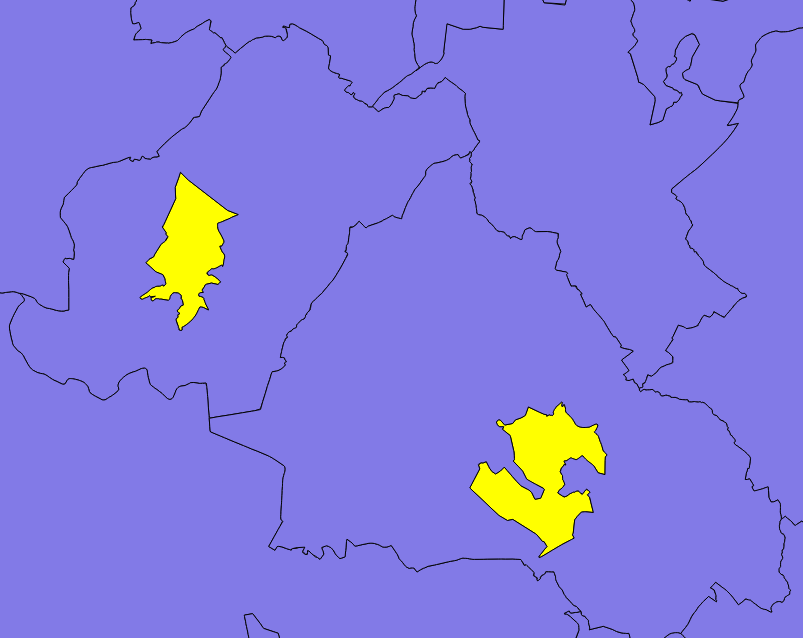
\includegraphics[width=0.4\linewidth]{images/ch6/innerRings}
\caption{Two examples of inner rings, highlighted in yellow.} \label{fig:rings}
\end{figure}

\begin{figure}[p]
\begin{tabularx}{1\textwidth}{XXXX}
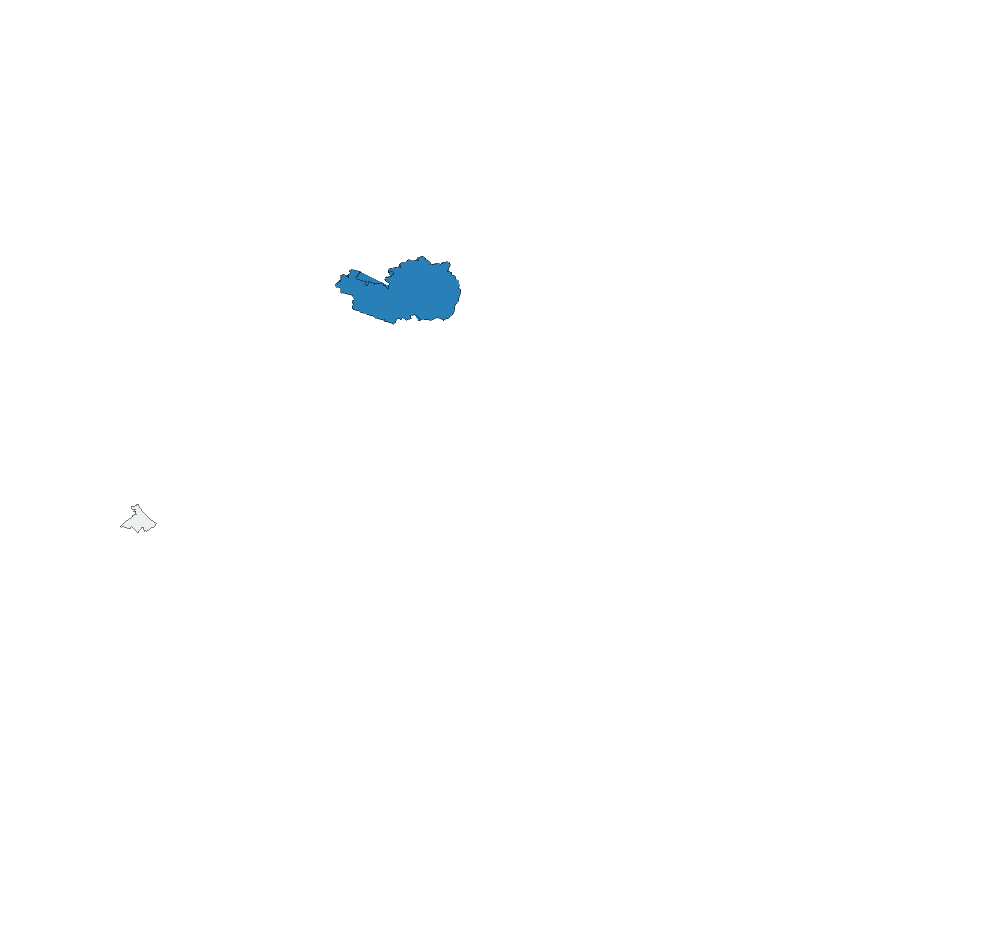
\includegraphics[width=1\linewidth]{images/ch6/loading/01}&
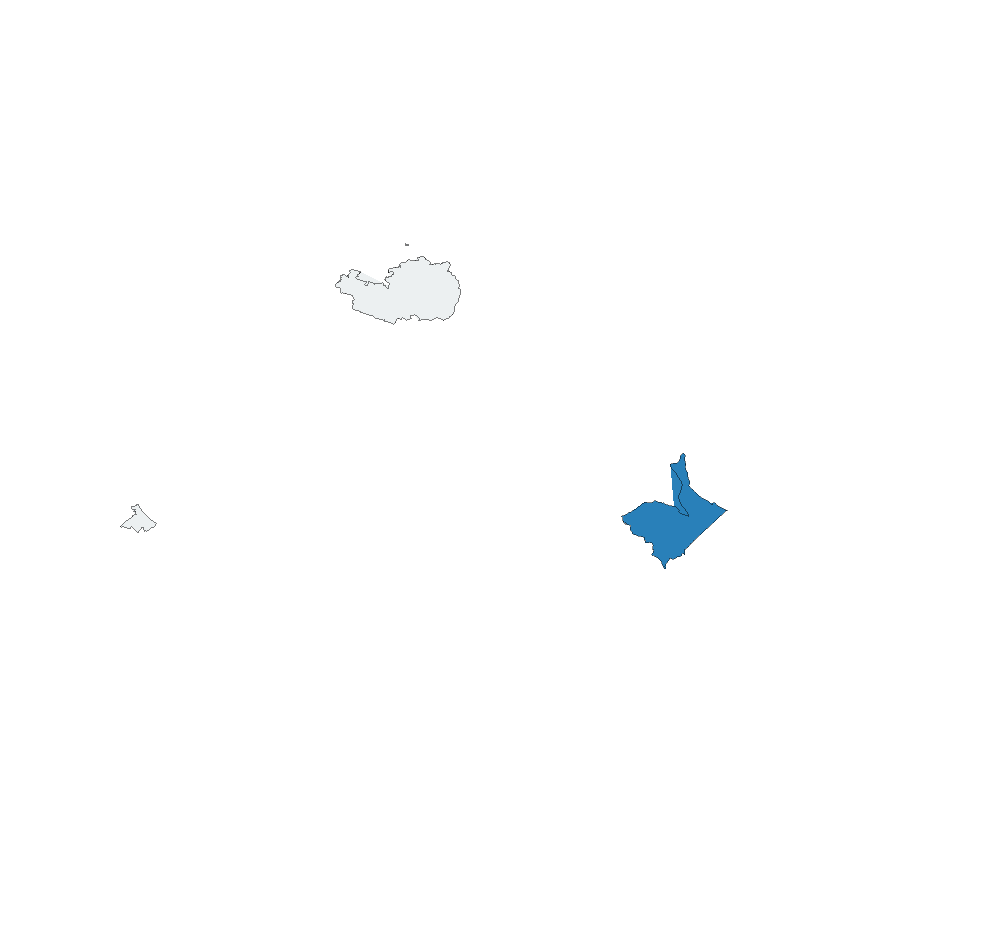
\includegraphics[width=1\linewidth]{images/ch6/loading/02}&
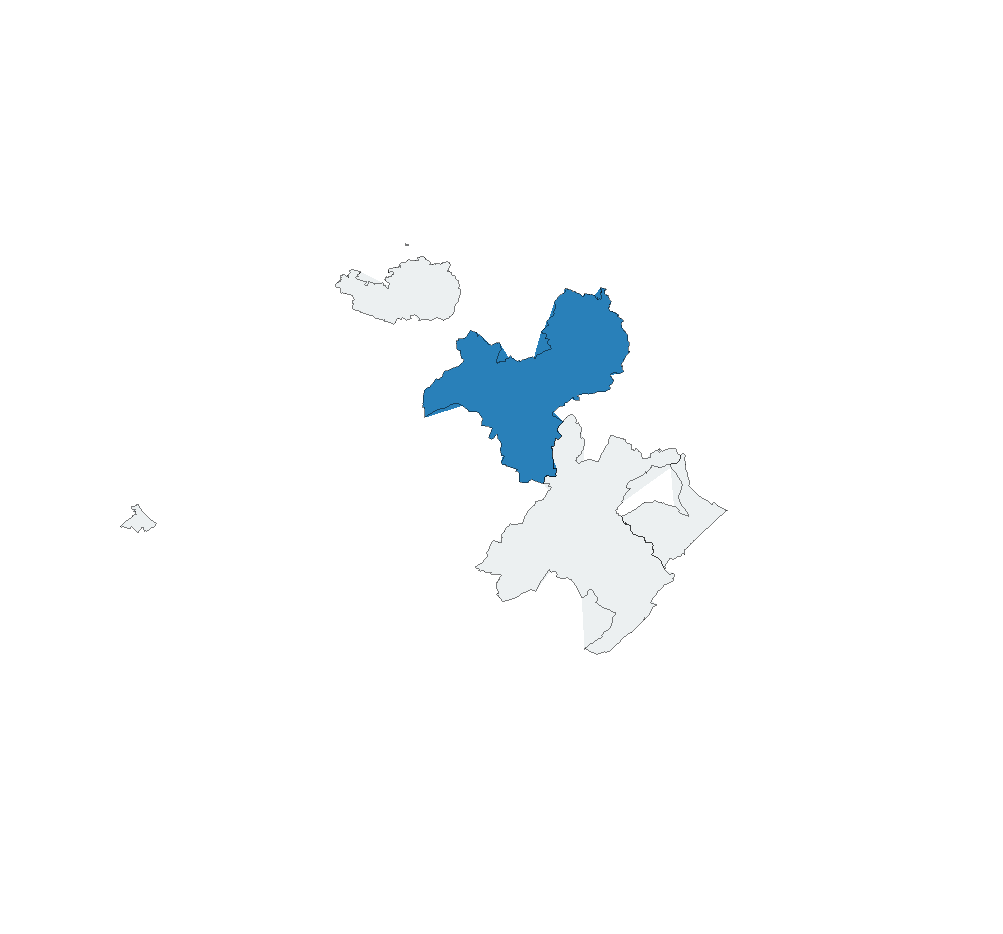
\includegraphics[width=1\linewidth]{images/ch6/loading/03}&
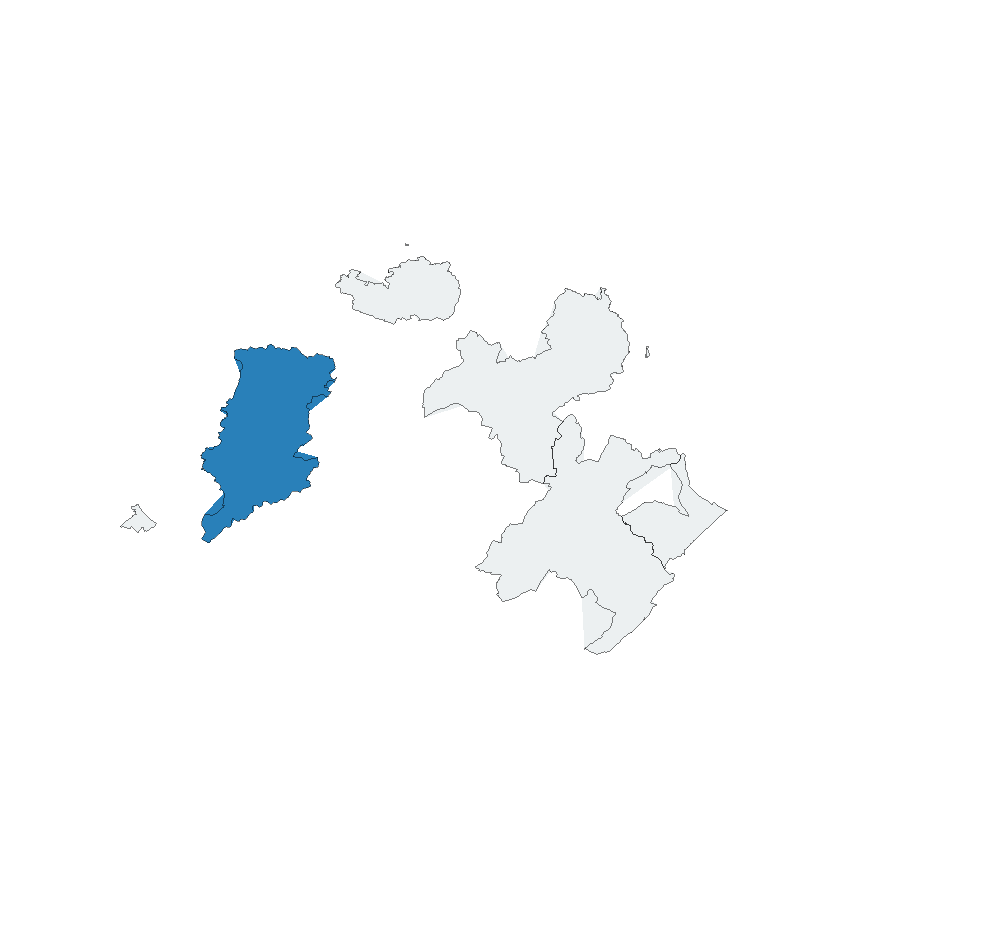
\includegraphics[width=1\linewidth]{images/ch6/loading/04} \\
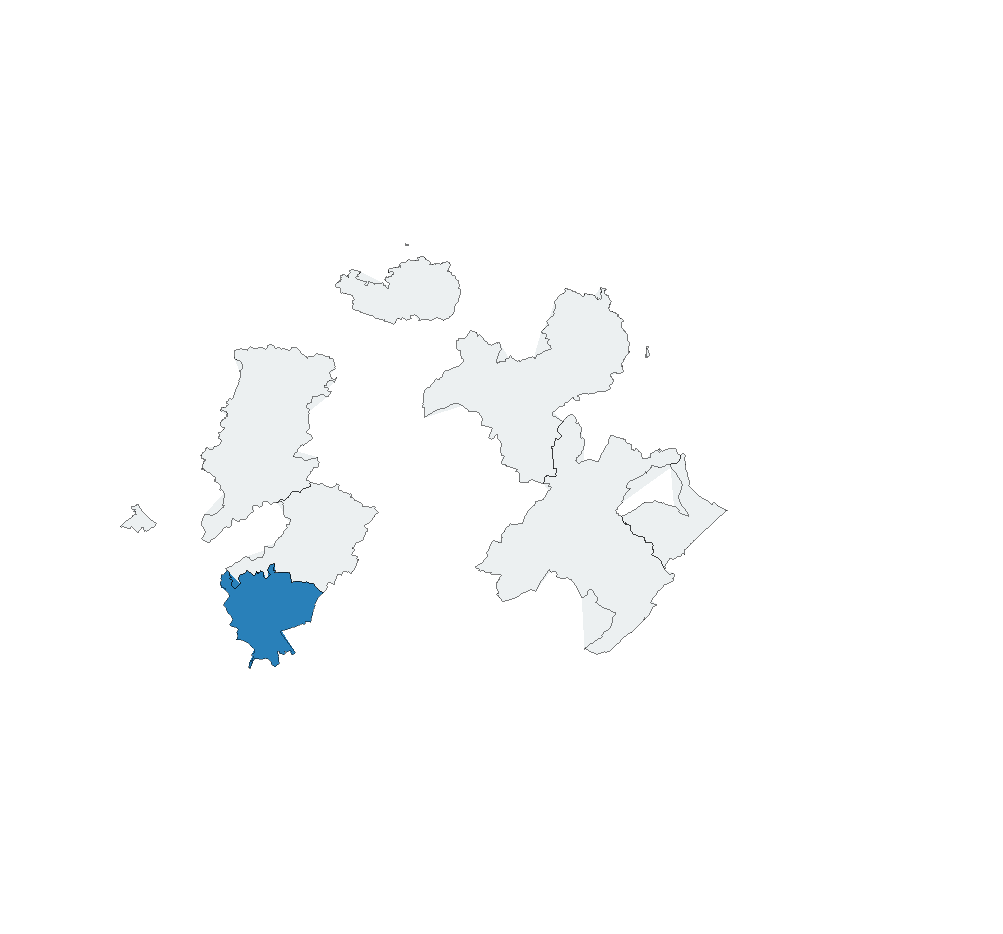
\includegraphics[width=1\linewidth]{images/ch6/loading/05}&
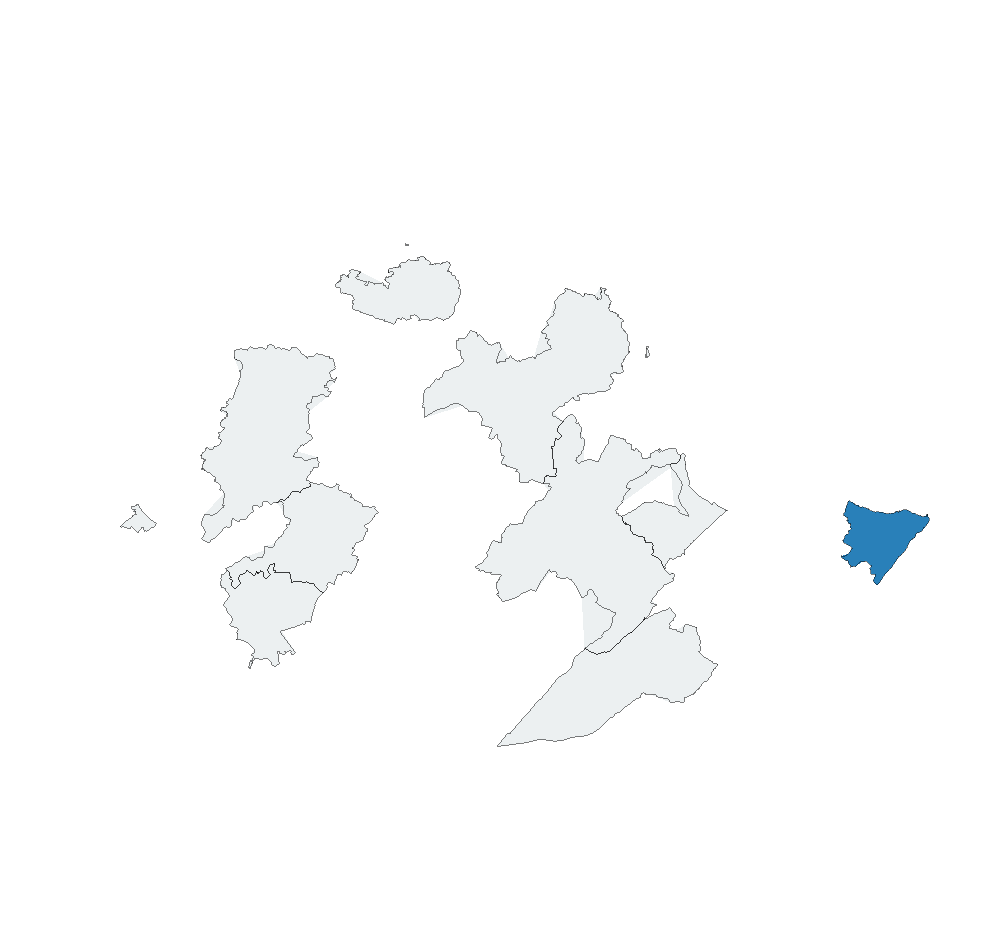
\includegraphics[width=1\linewidth]{images/ch6/loading/06}&
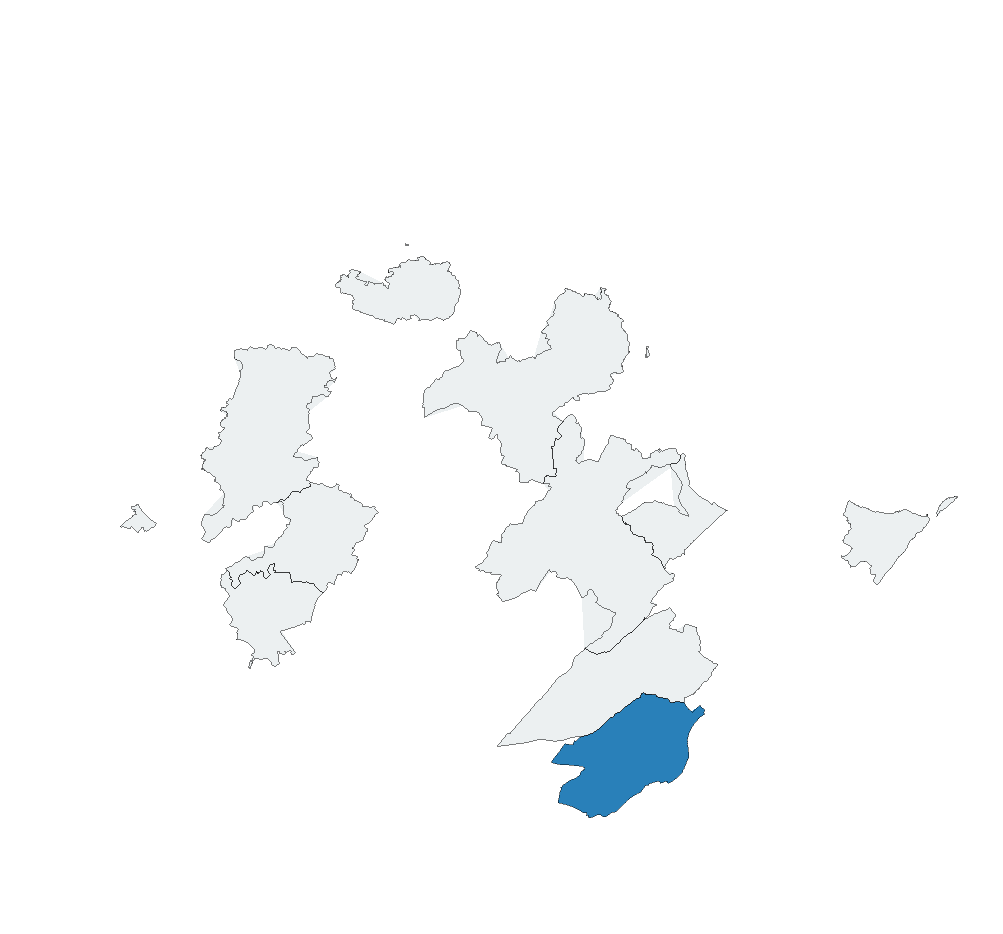
\includegraphics[width=1\linewidth]{images/ch6/loading/07}&
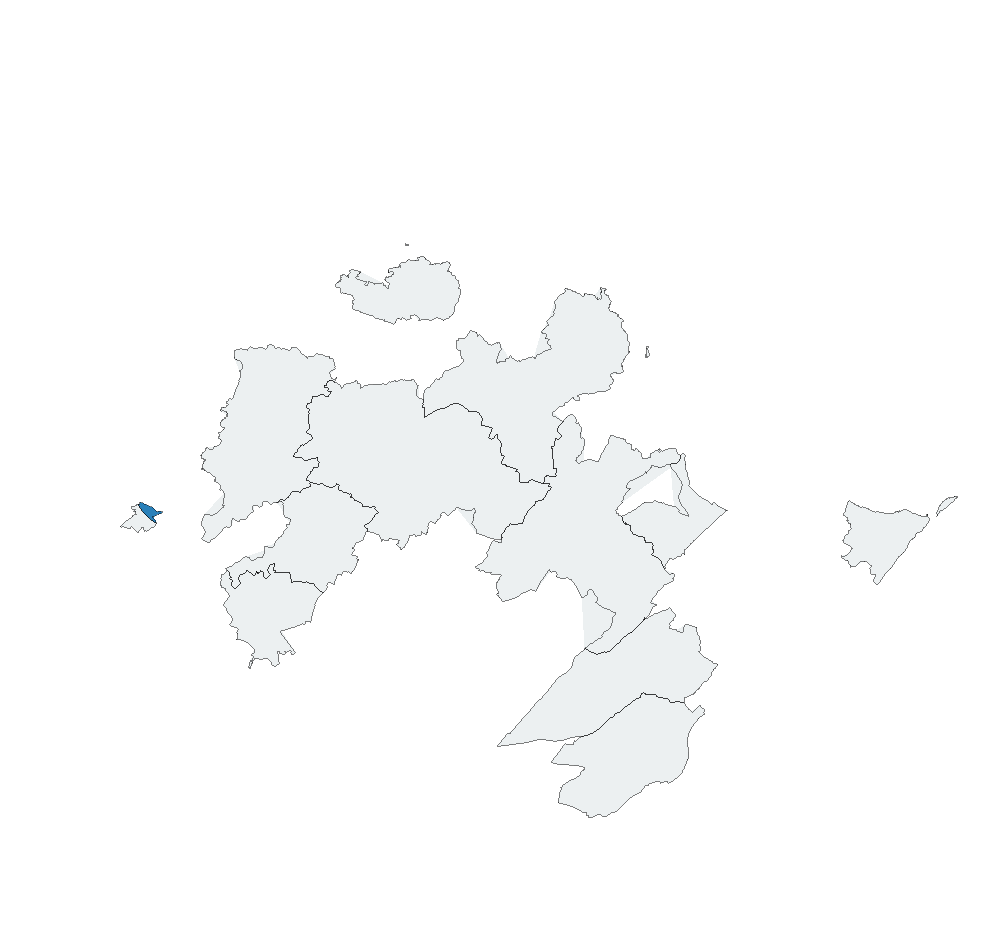
\includegraphics[width=1\linewidth]{images/ch6/loading/08} \\
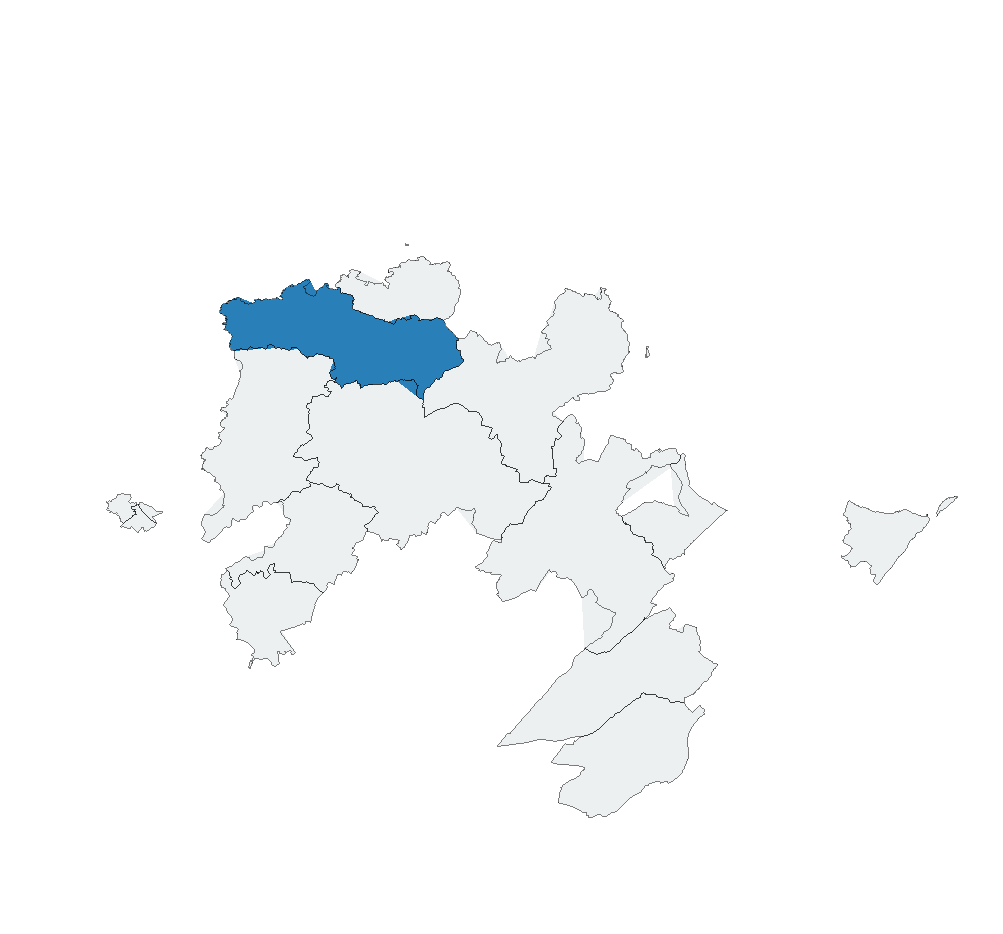
\includegraphics[width=1\linewidth]{images/ch6/loading/09}&
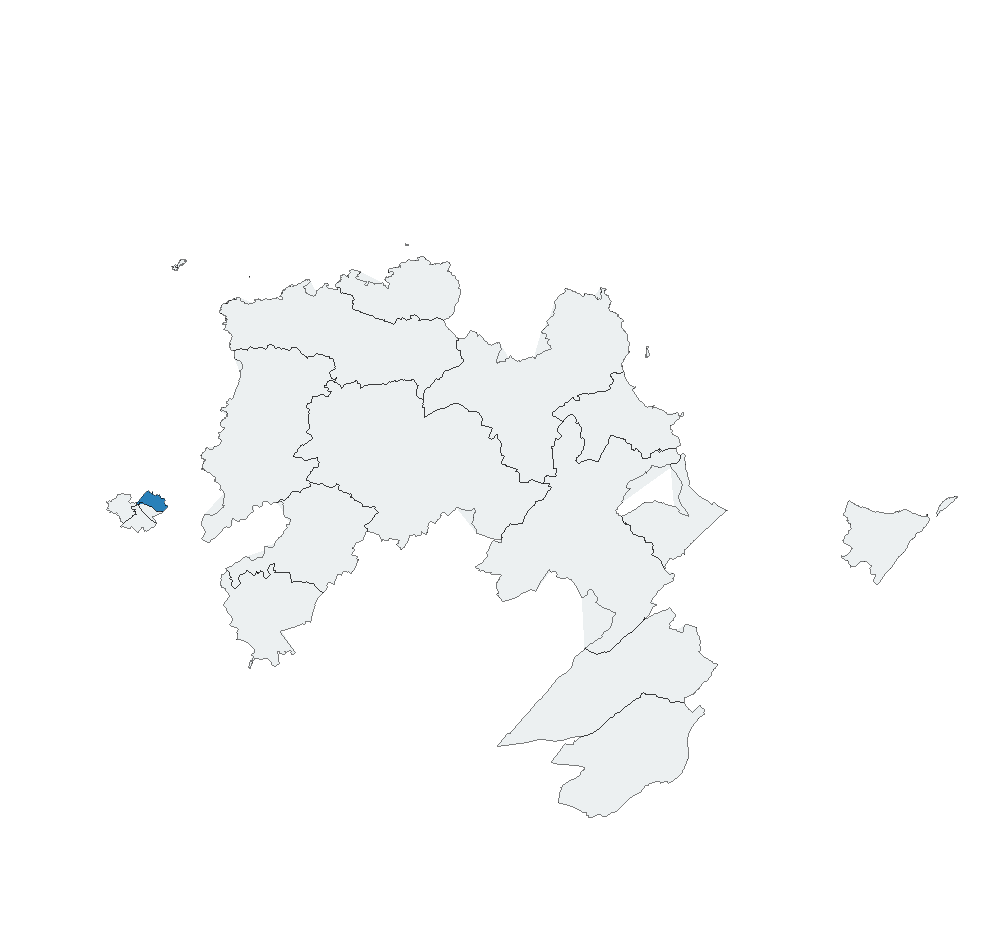
\includegraphics[width=1\linewidth]{images/ch6/loading/10}&
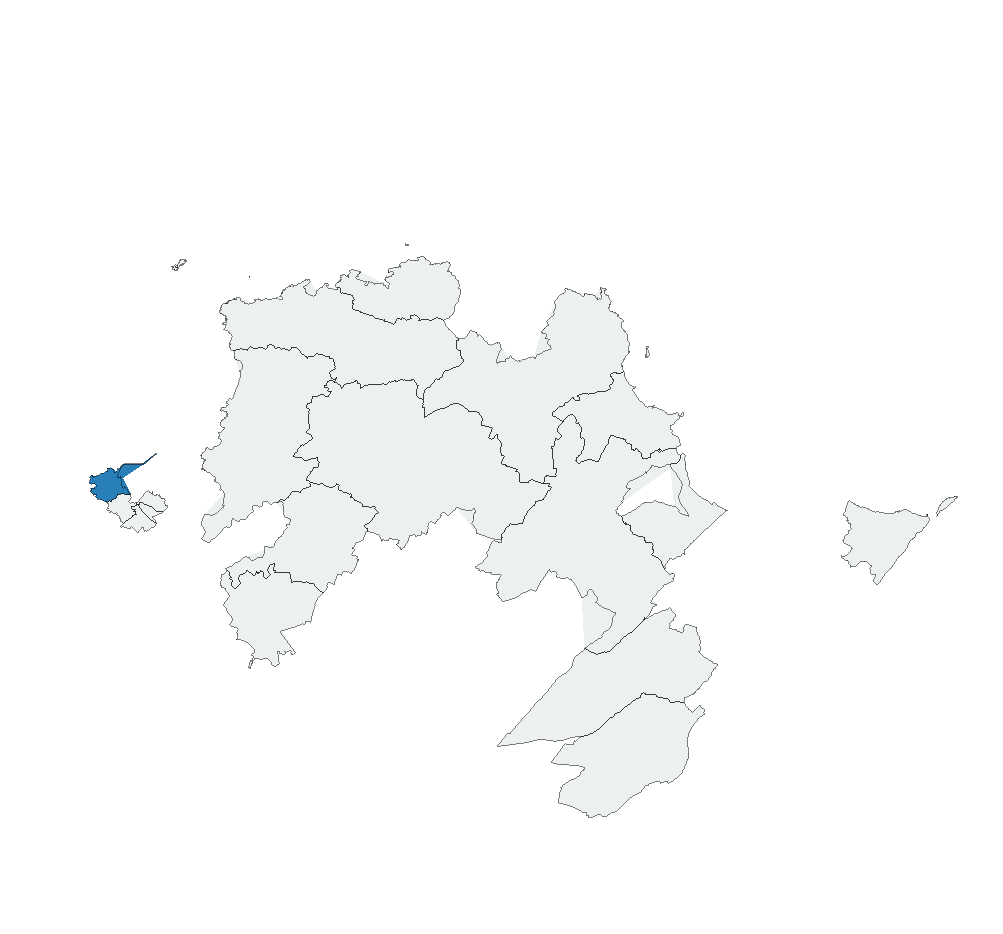
\includegraphics[width=1\linewidth]{images/ch6/loading/11}&
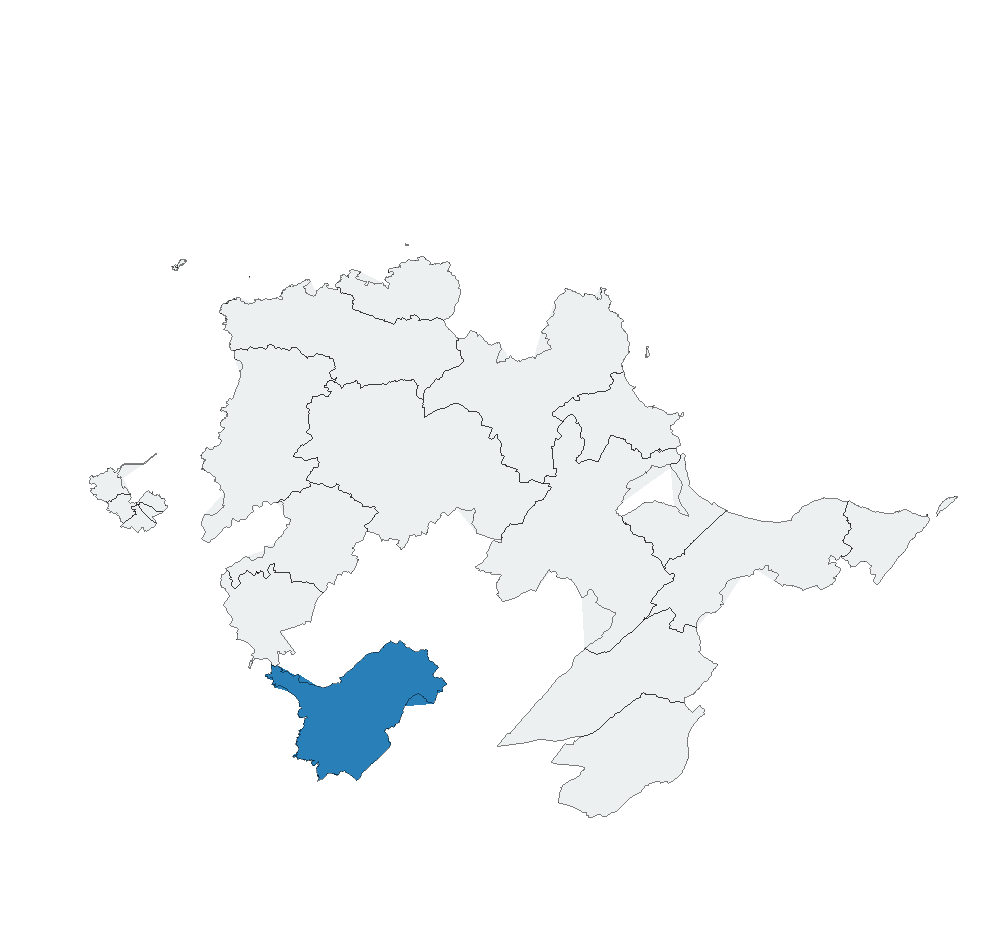
\includegraphics[width=1\linewidth]{images/ch6/loading/12} \\
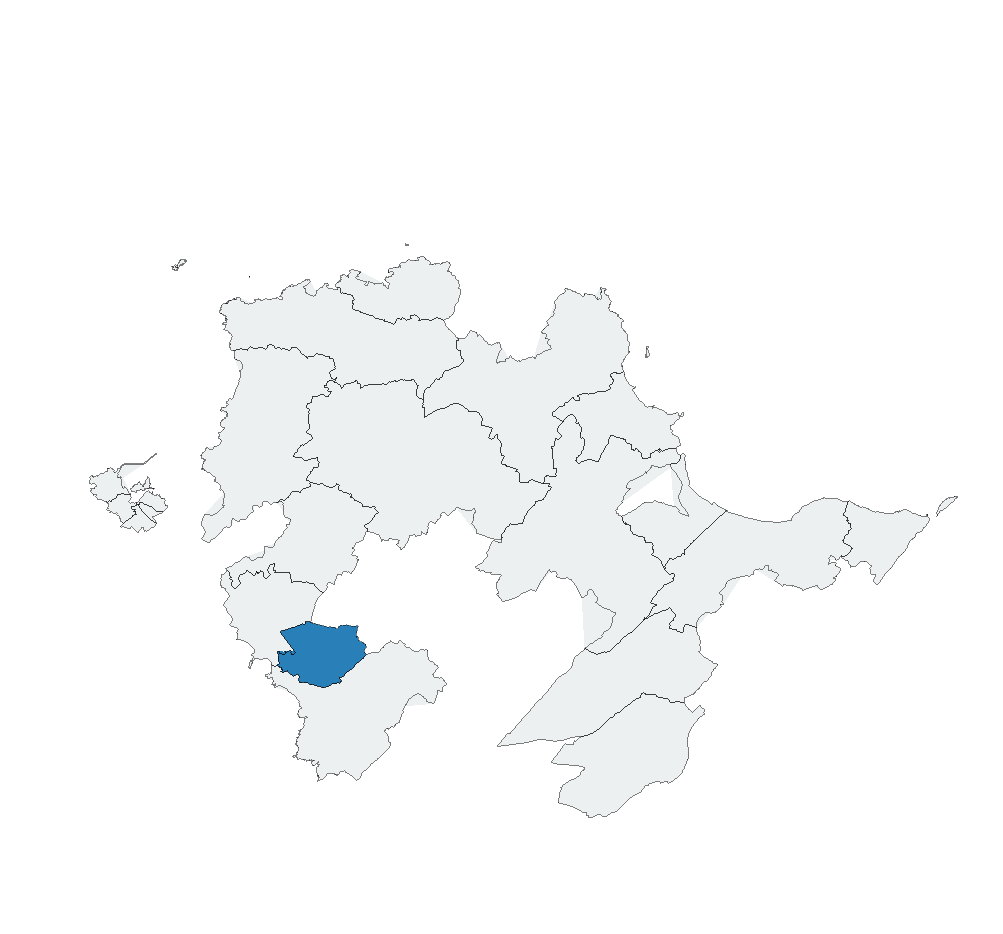
\includegraphics[width=1\linewidth]{images/ch6/loading/13}&
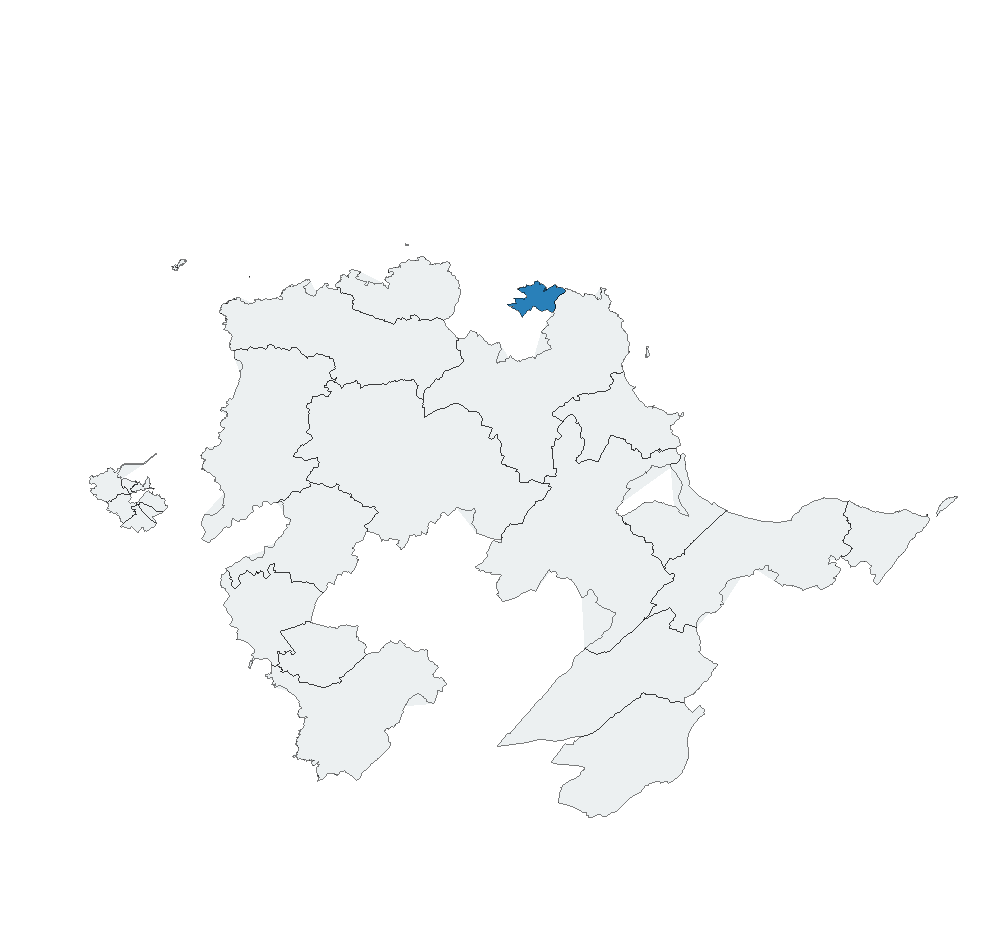
\includegraphics[width=1\linewidth]{images/ch6/loading/14}&
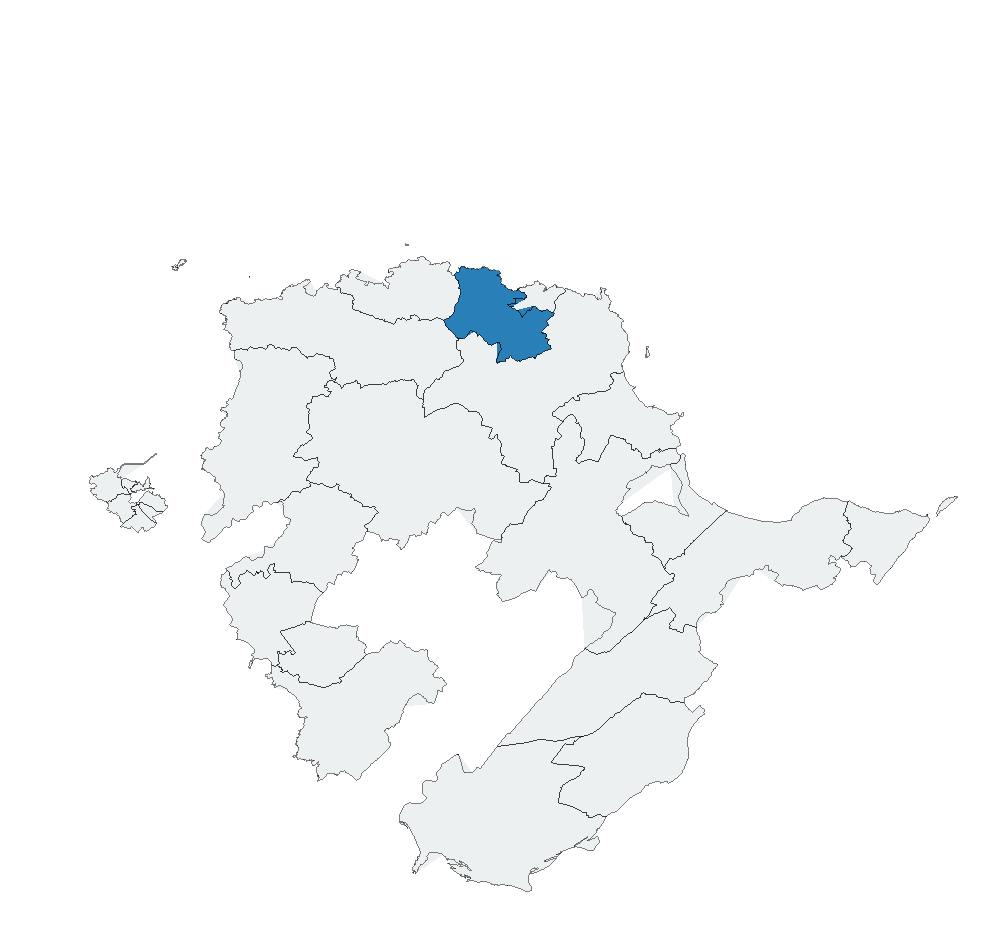
\includegraphics[width=1\linewidth]{images/ch6/loading/15}&
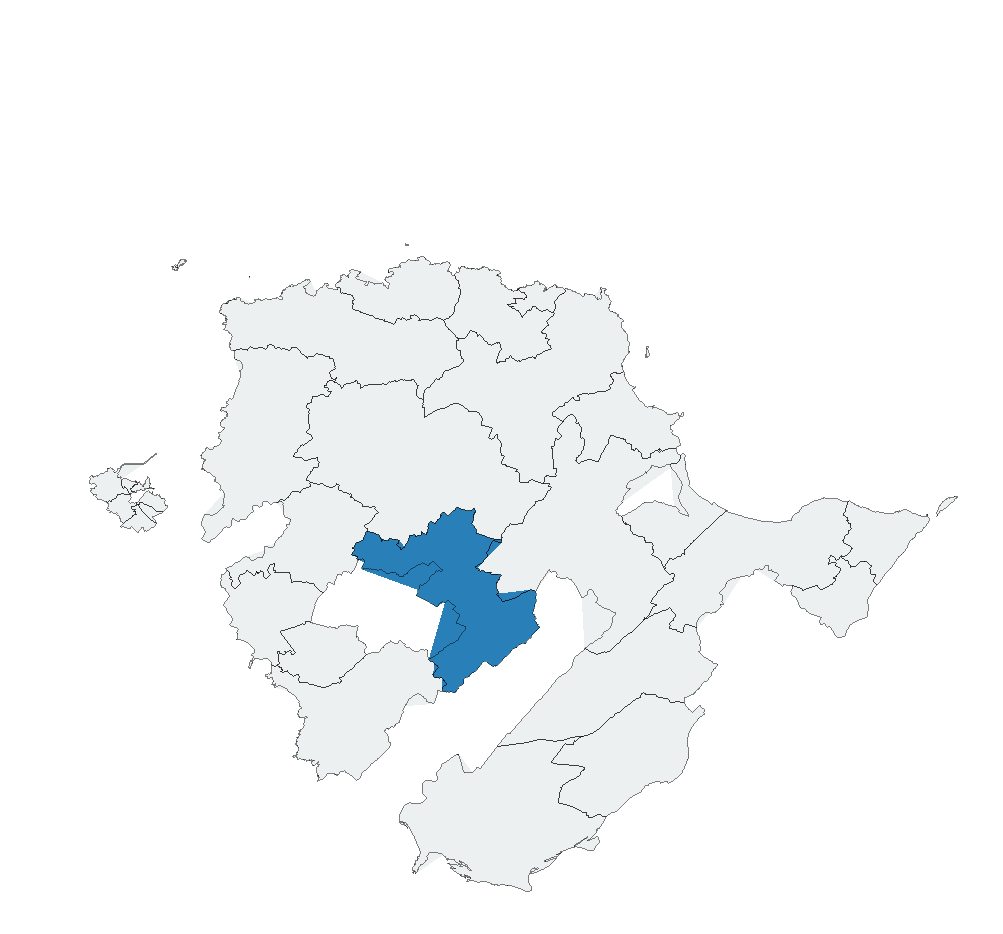
\includegraphics[width=1\linewidth]{images/ch6/loading/16} \\
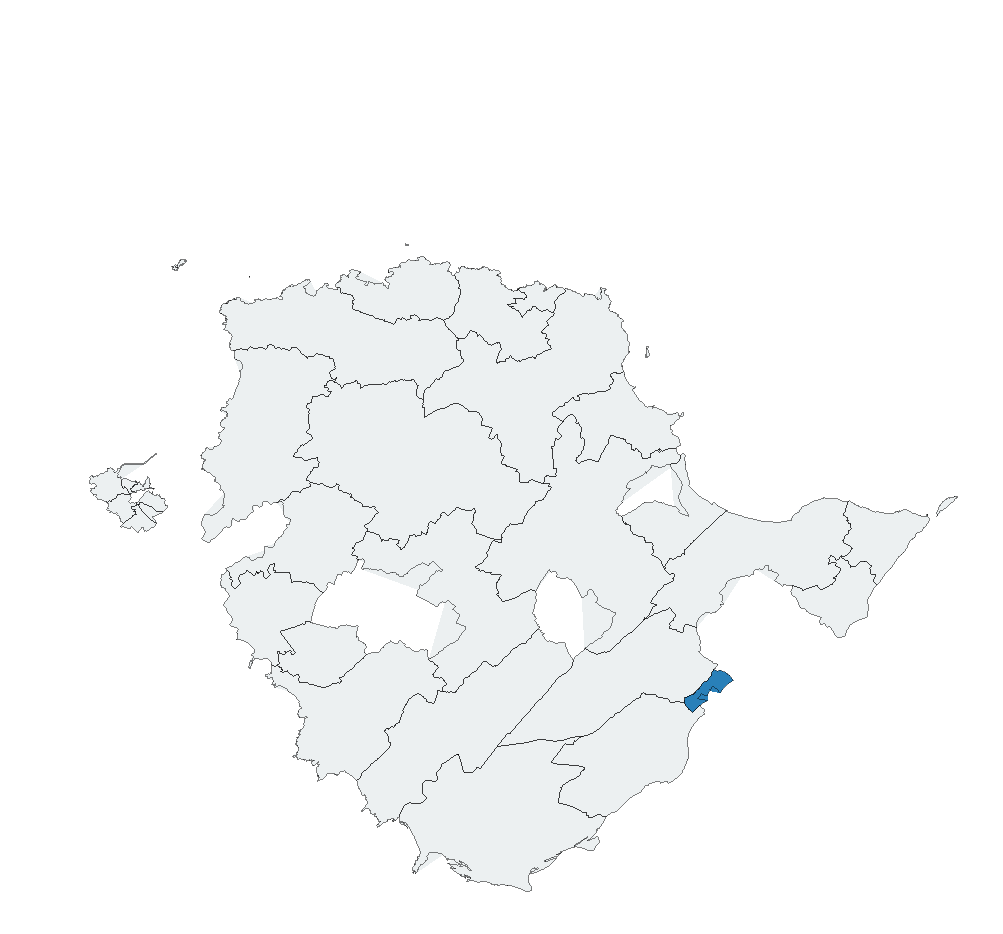
\includegraphics[width=1\linewidth]{images/ch6/loading/17}&
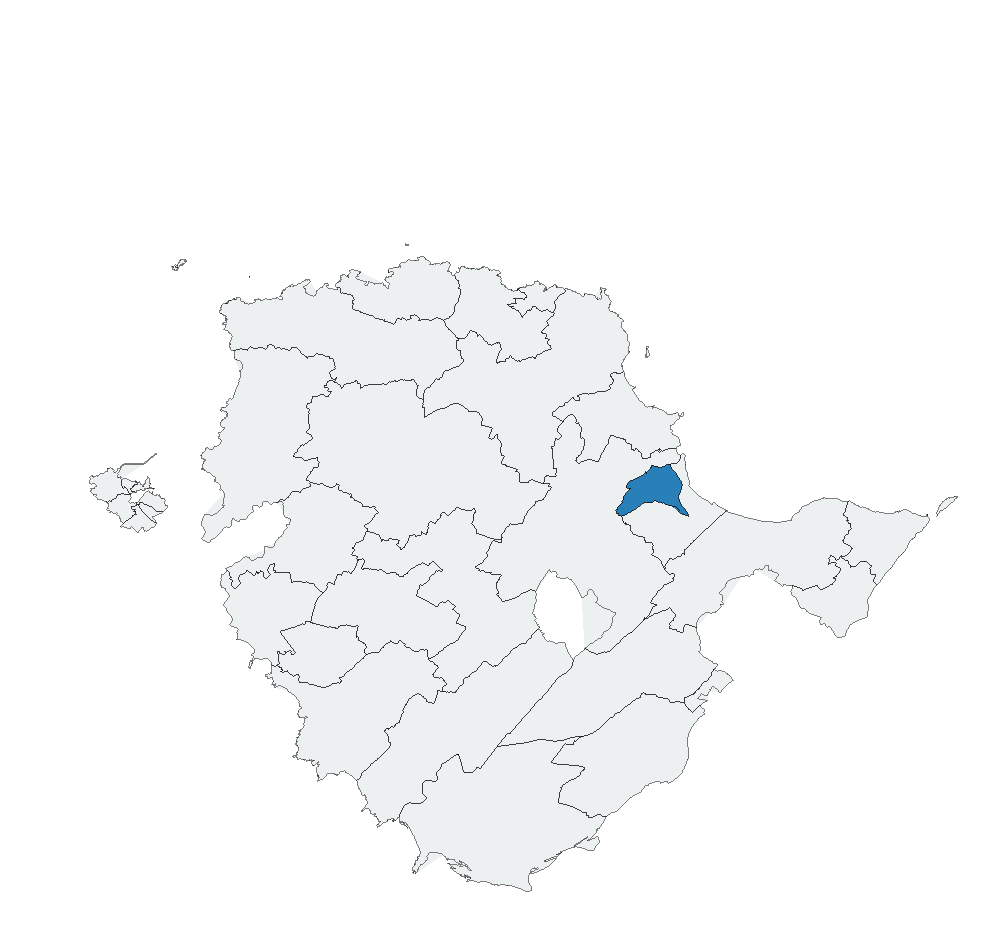
\includegraphics[width=1\linewidth]{images/ch6/loading/18}&
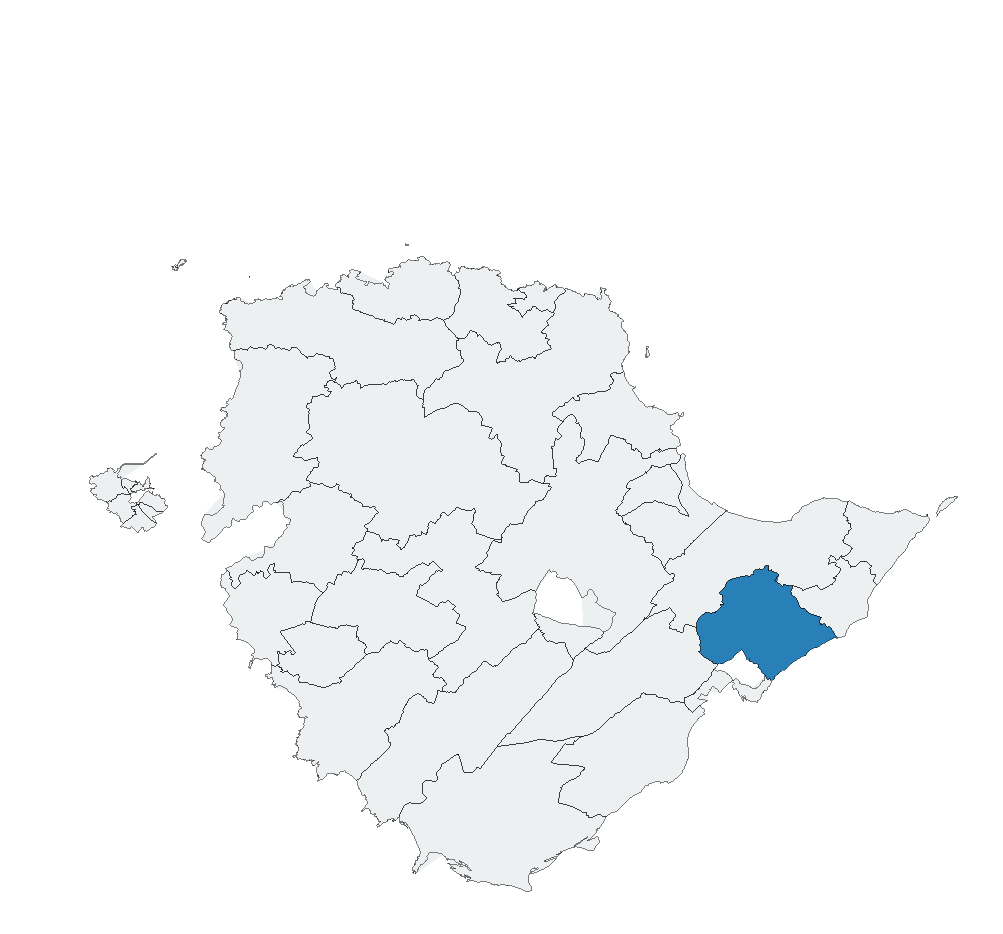
\includegraphics[width=1\linewidth]{images/ch6/loading/19}&
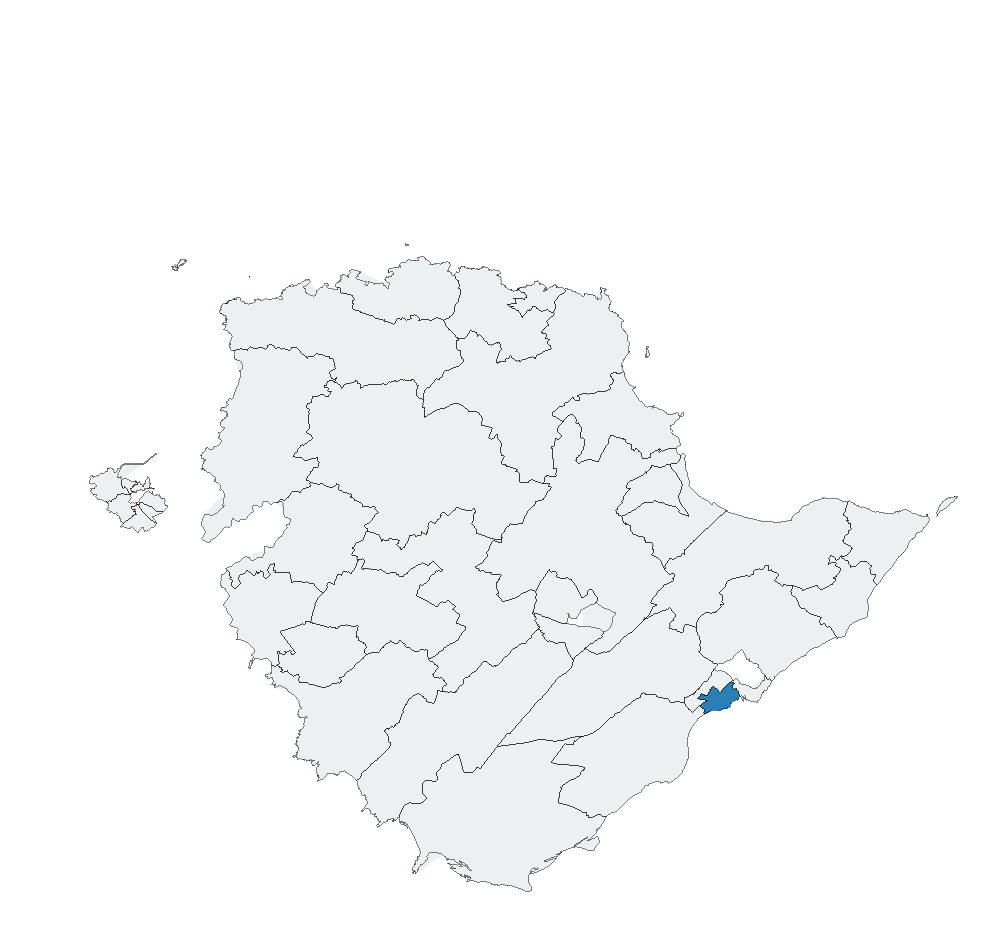
\includegraphics[width=1\linewidth]{images/ch6/loading/20} \\
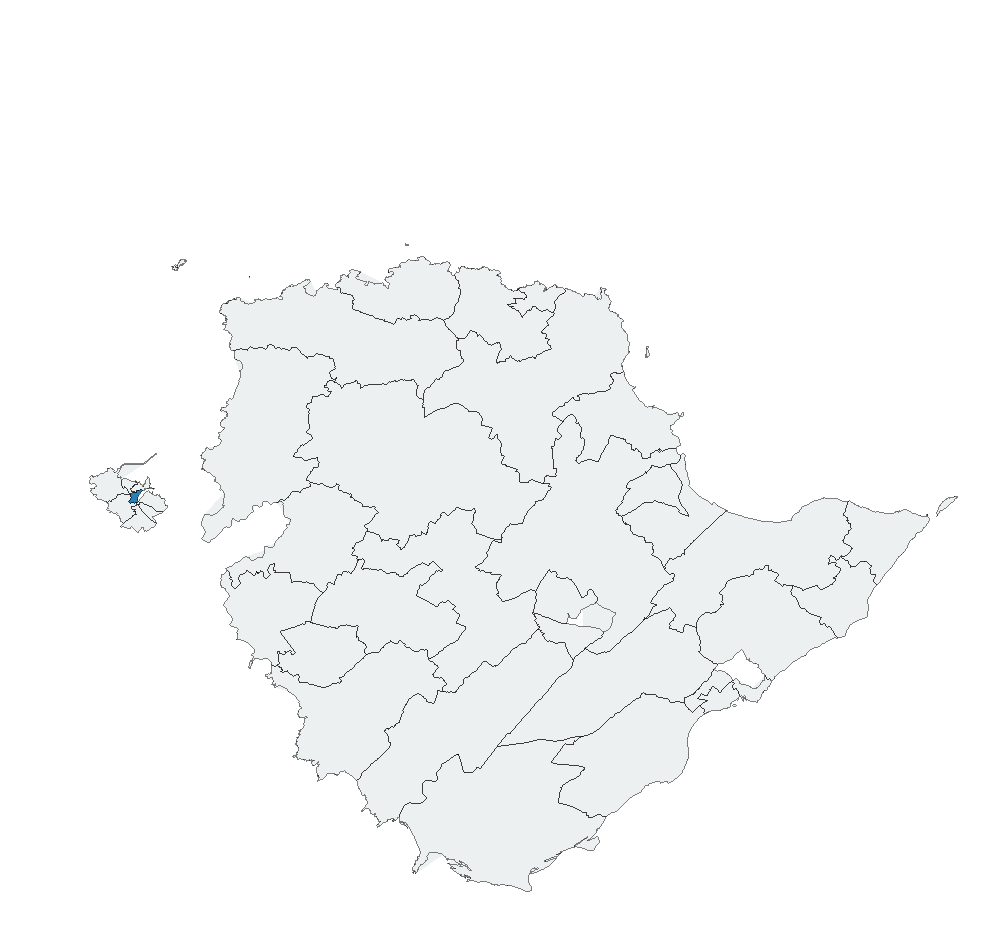
\includegraphics[width=1\linewidth]{images/ch6/loading/21}&
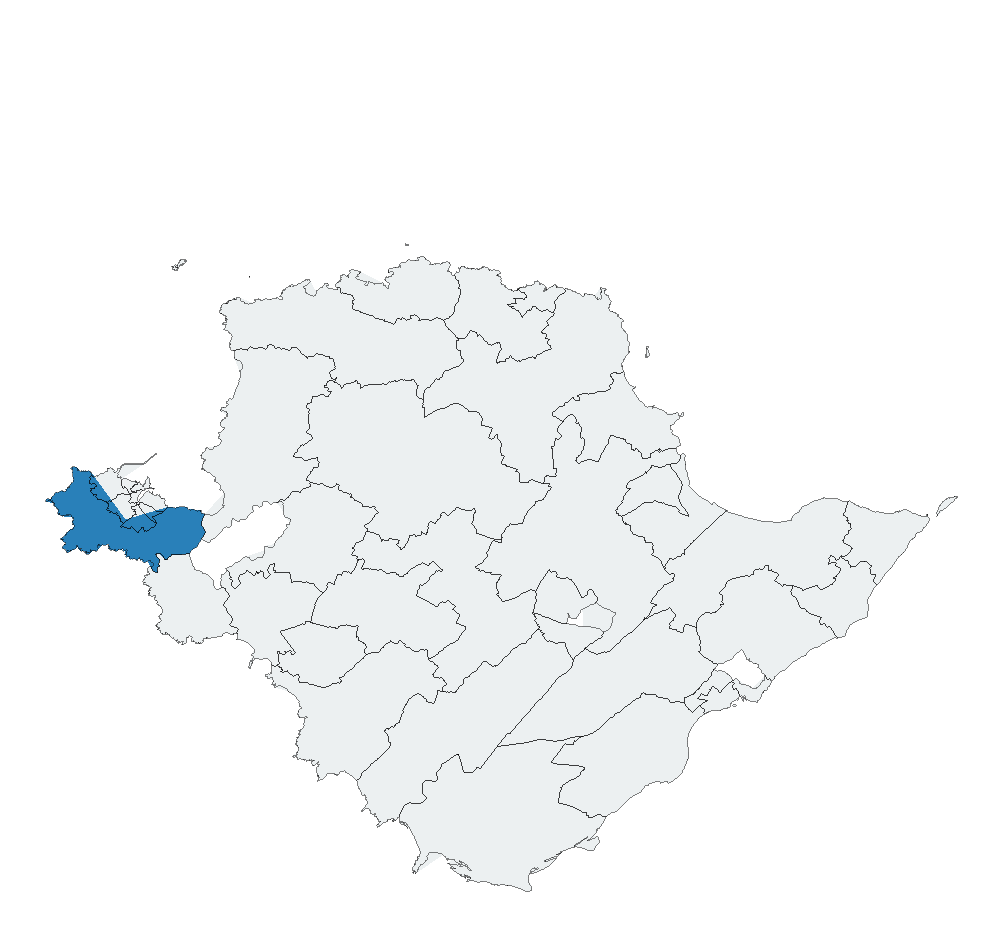
\includegraphics[width=1\linewidth]{images/ch6/loading/22}&
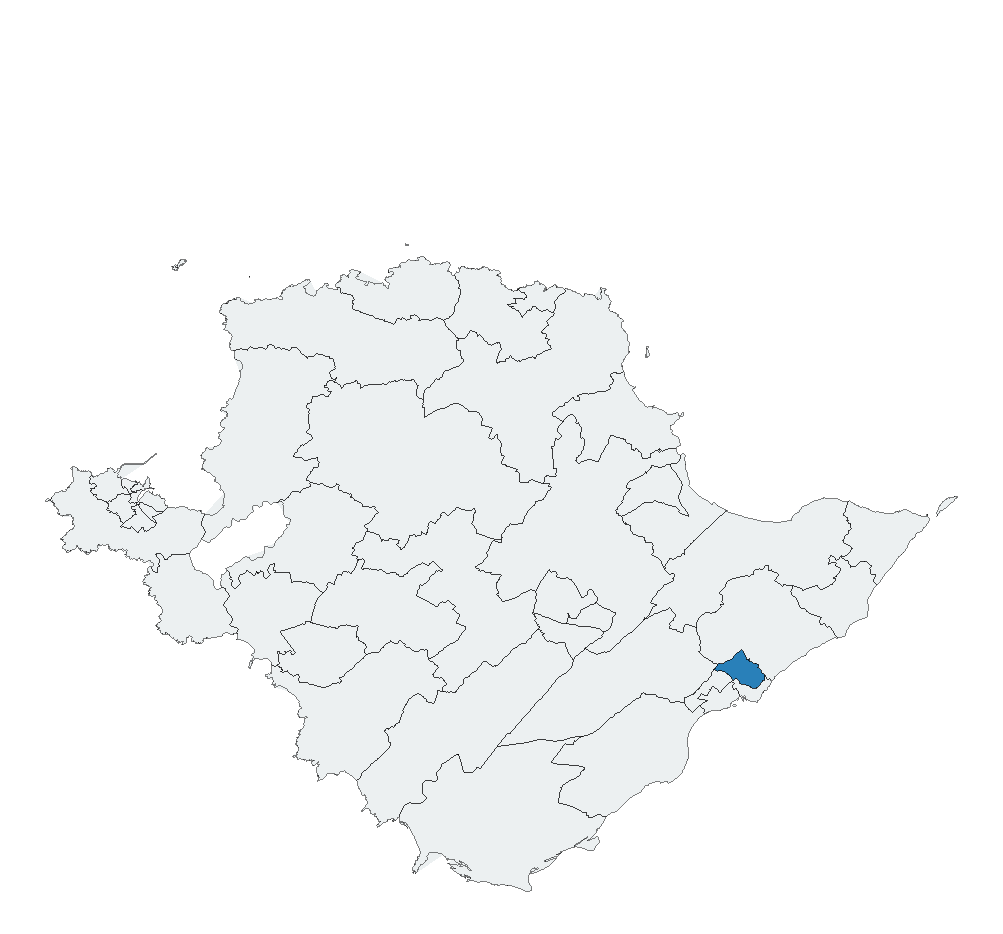
\includegraphics[width=1\linewidth]{images/ch6/loading/23}&
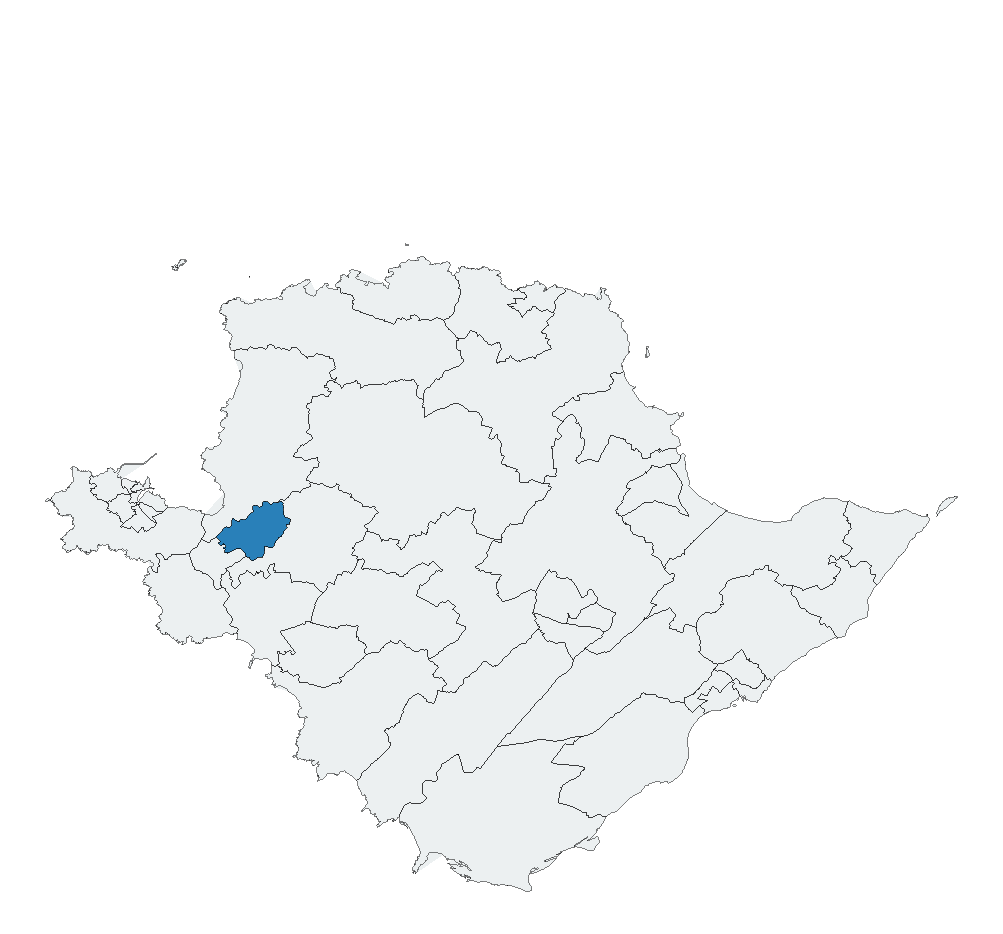
\includegraphics[width=1\linewidth]{images/ch6/loading/24} \\ %24
\end{tabularx}
\caption{A matrix depicting time slices of the temporal debug visualization for geospatial debug loading. The blue presents the last loaded polygon, whilst they grey represent polygons that have already been loaded.} \label{fig:loadingMatrix}
\end{figure}

These mistakes may have been avoided by a more experienced user of the library, but geospatial debug visualization proved an essential tool for new users.

\subsection{Contiguity Visualization} \label{sec:contigVis}
We reduce the complexity of hierarchy building by introducing a constraint that all hierarchies are complete when exactly one area remains in our merge candidate list. In order to do this, we need to make sure that every instance of the hierarchy is formed one contiguous region. We debug this aspect by mapping a random color to each list of polygons (representing a contiguous region) at each intermediate step, where a step is presented when each polygon has its contiguity tested. As there may be an arbitrary number of contiguous regions, designating identifiable colors is difficult. Therefore, in order to address this challenge, we altered the program slightly. When a polygon is assigned to a contiguous region, a new color is assigned to the region, This allows for a visible understanding of the change without the need for the step function. We present a matrix of images showing a concise contiguity visualization in Figure \ref{fig:contigMatrix}. 

\begin{figure}[p]
\begin{tabularx}{1\textwidth}{XXXX}
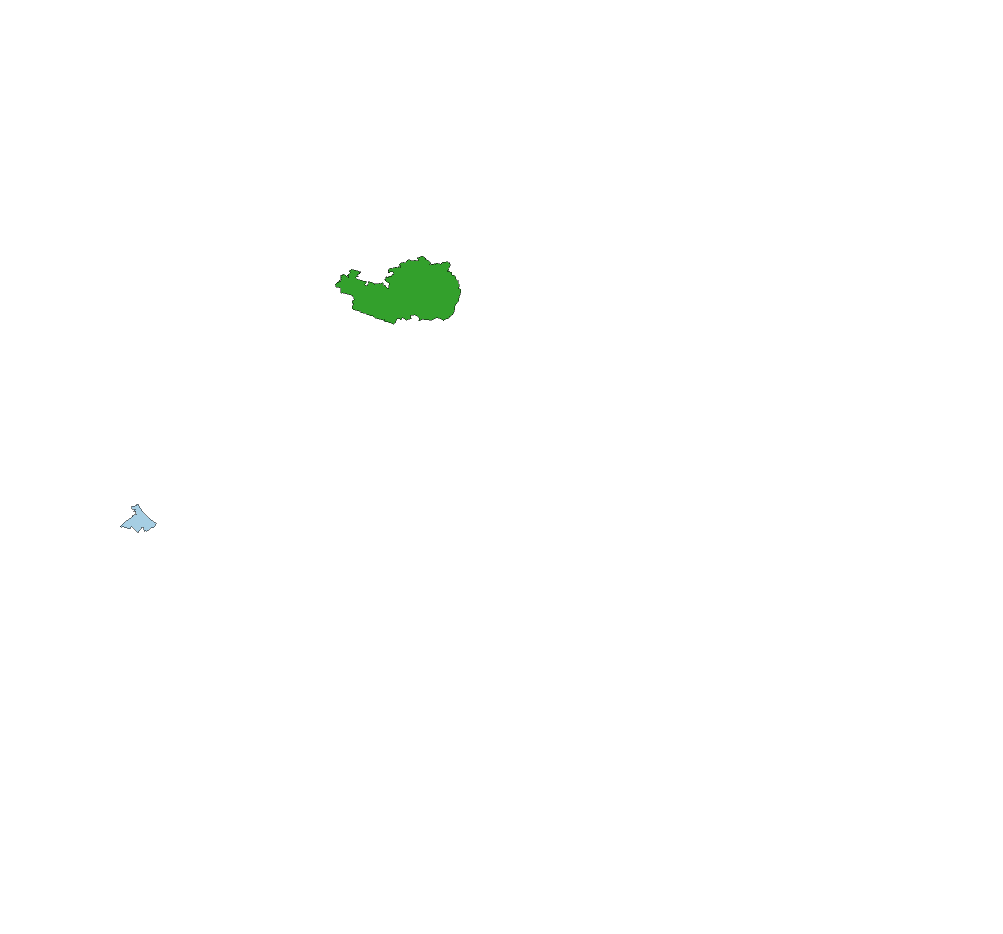
\includegraphics[width=1\linewidth]{images/ch6/contig/01}&
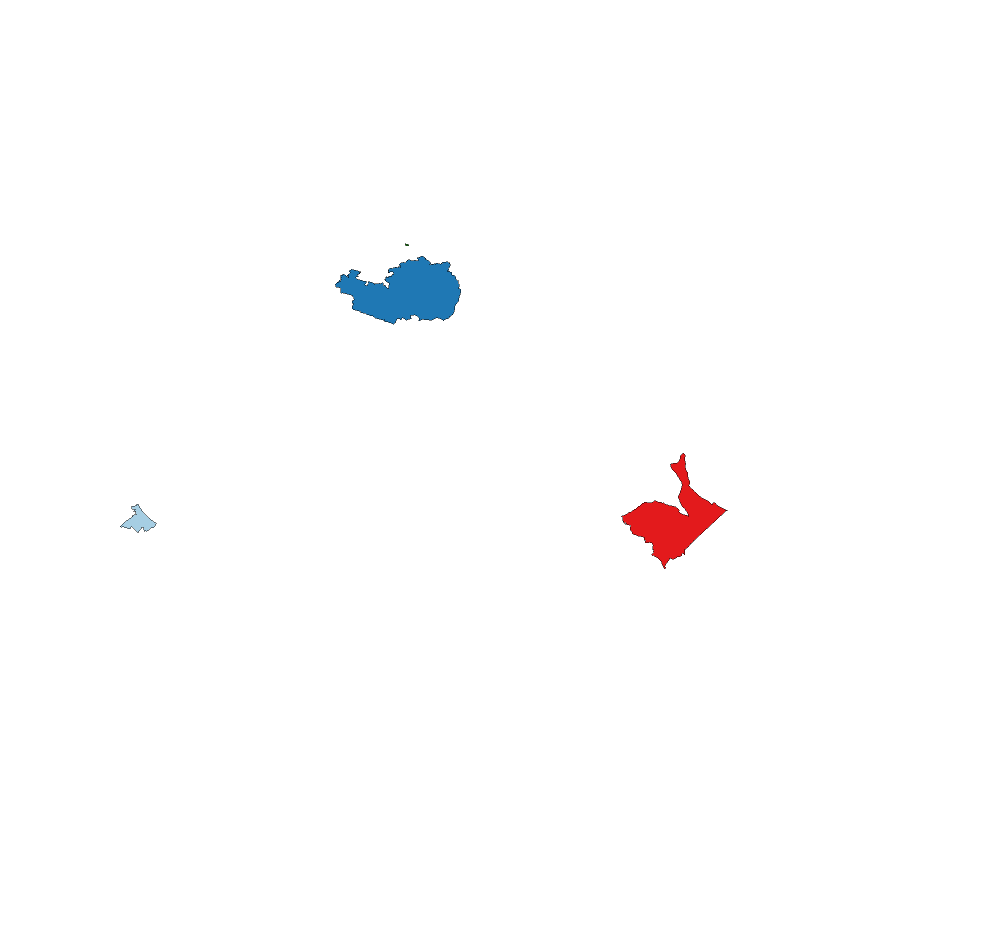
\includegraphics[width=1\linewidth]{images/ch6/contig/02}&
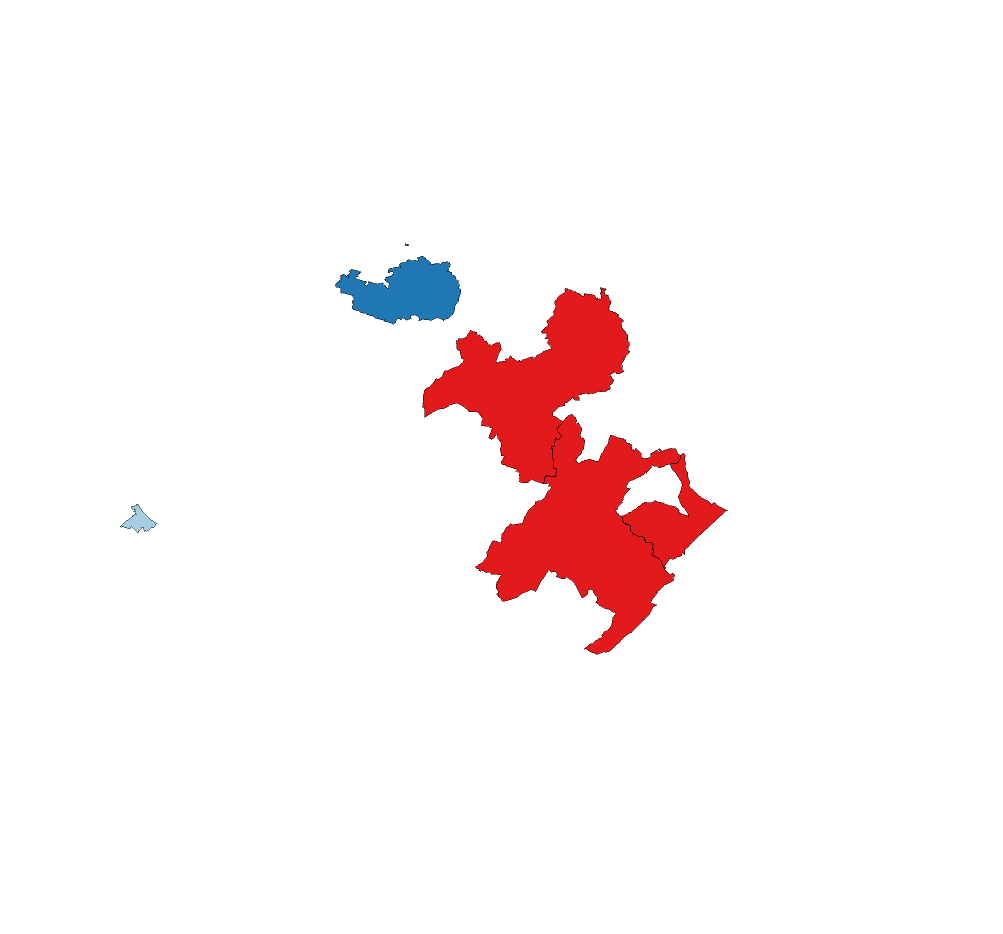
\includegraphics[width=1\linewidth]{images/ch6/contig/03}&
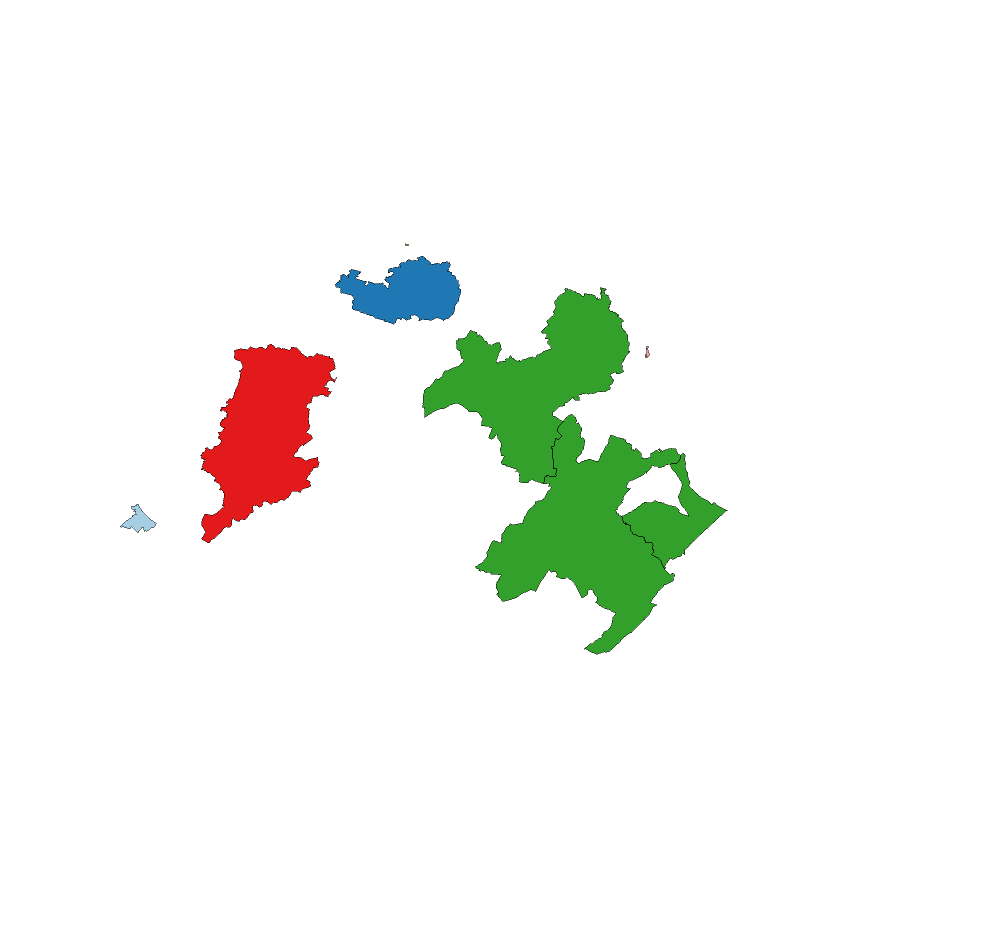
\includegraphics[width=1\linewidth]{images/ch6/contig/04} \\
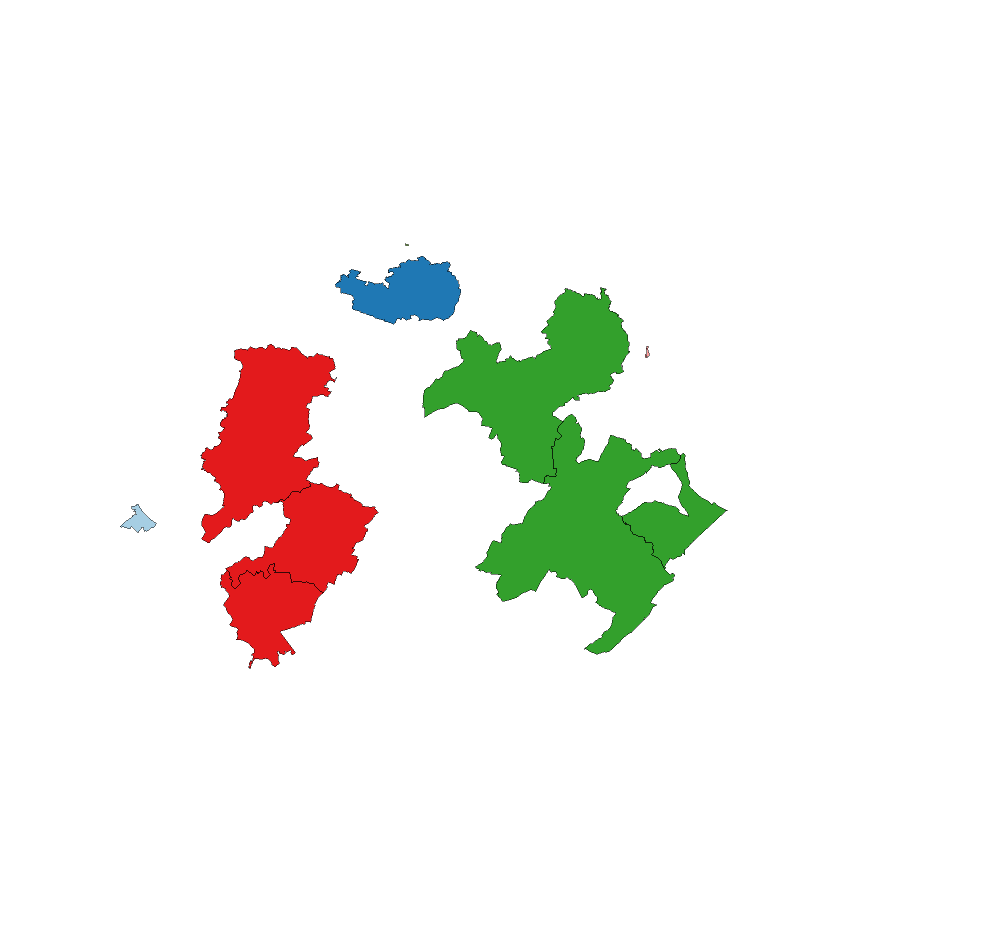
\includegraphics[width=1\linewidth]{images/ch6/contig/05}&
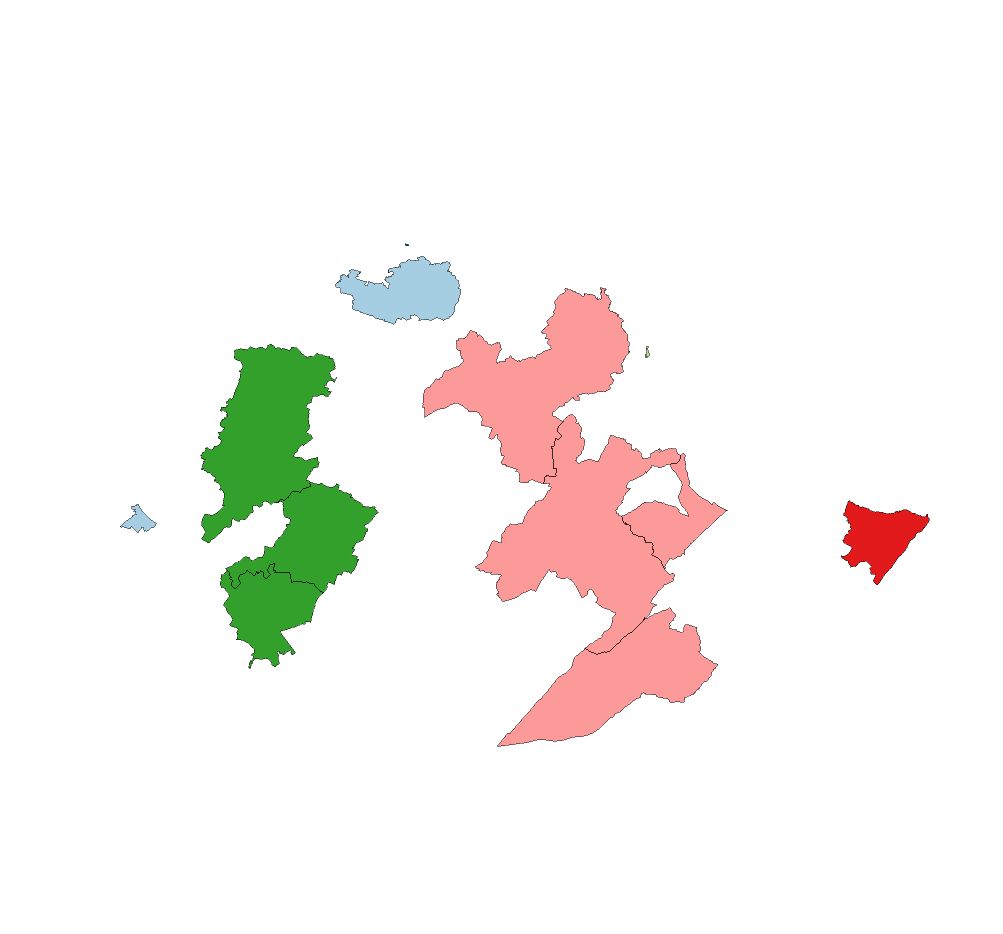
\includegraphics[width=1\linewidth]{images/ch6/contig/06}&
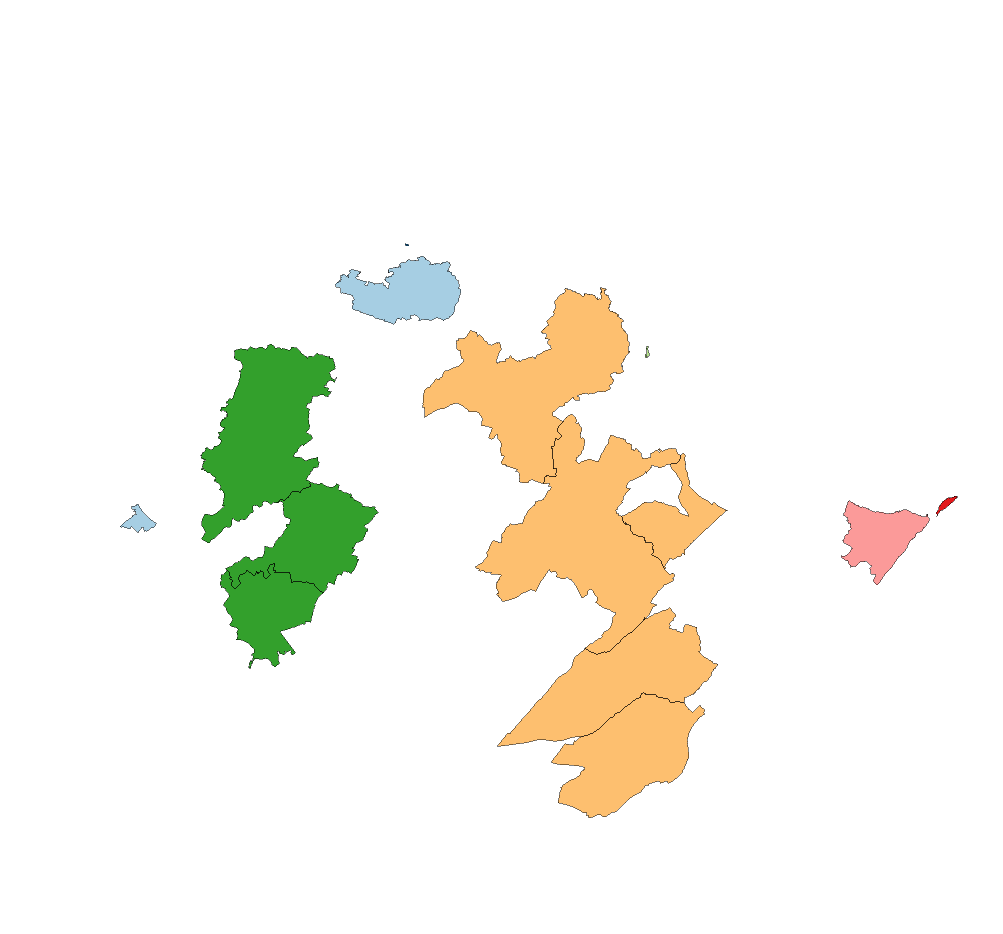
\includegraphics[width=1\linewidth]{images/ch6/contig/07}&
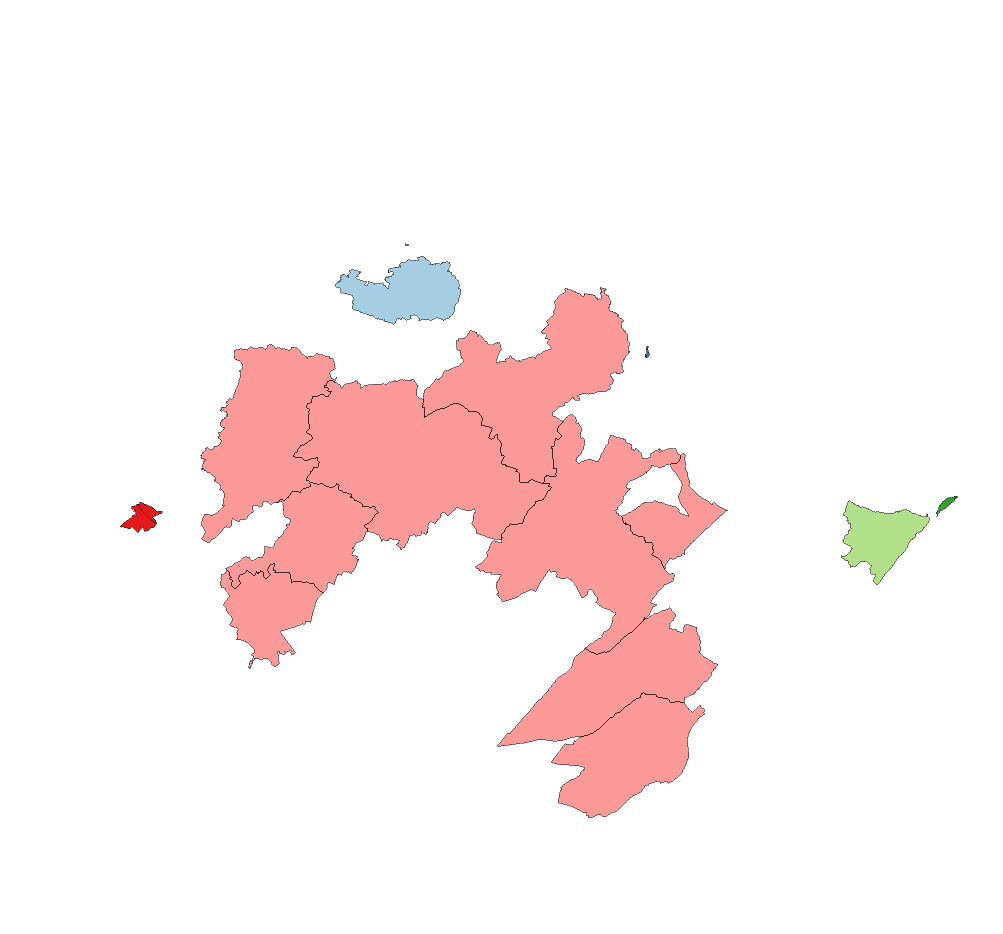
\includegraphics[width=1\linewidth]{images/ch6/contig/08} \\
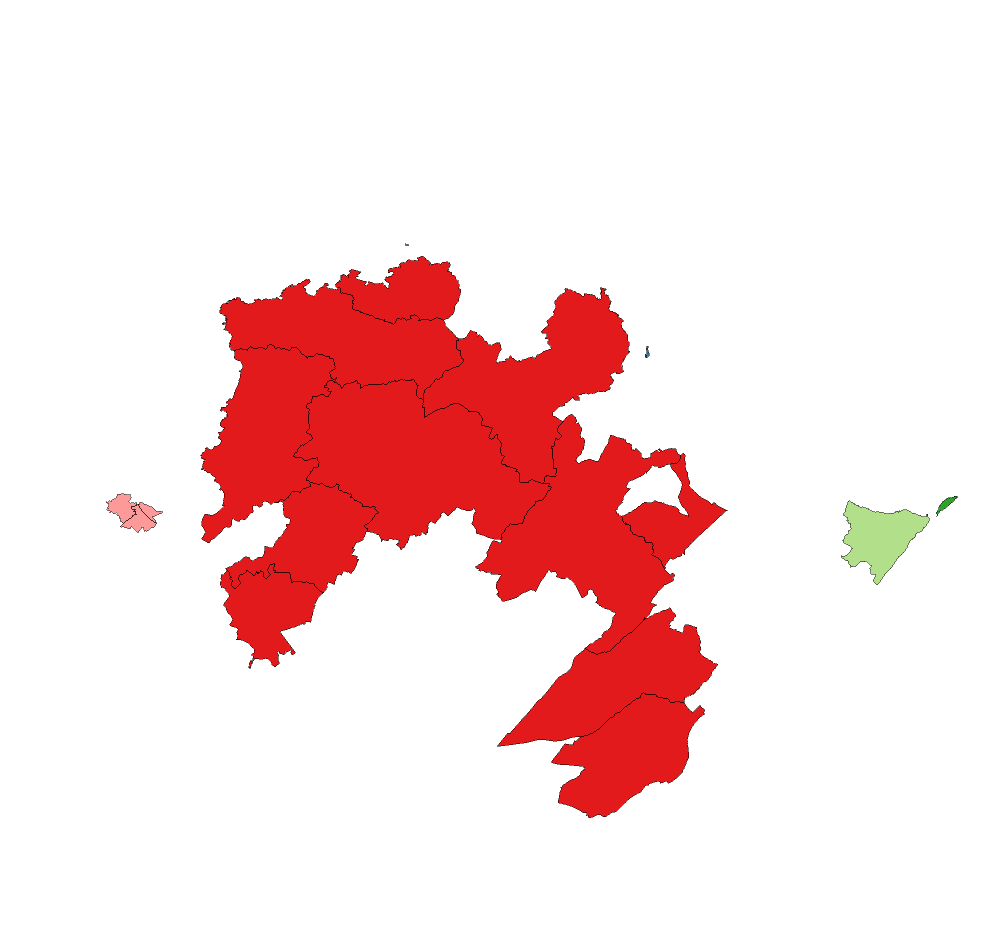
\includegraphics[width=1\linewidth]{images/ch6/contig/09}&
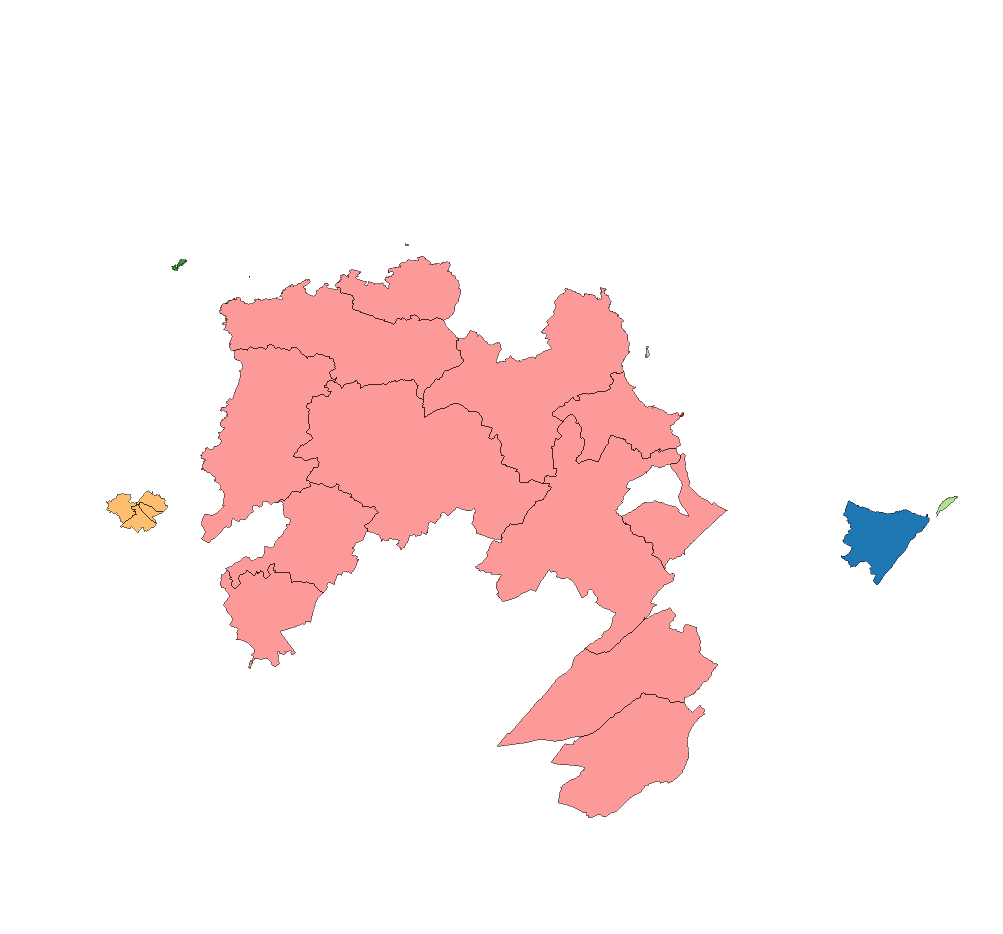
\includegraphics[width=1\linewidth]{images/ch6/contig/10}&
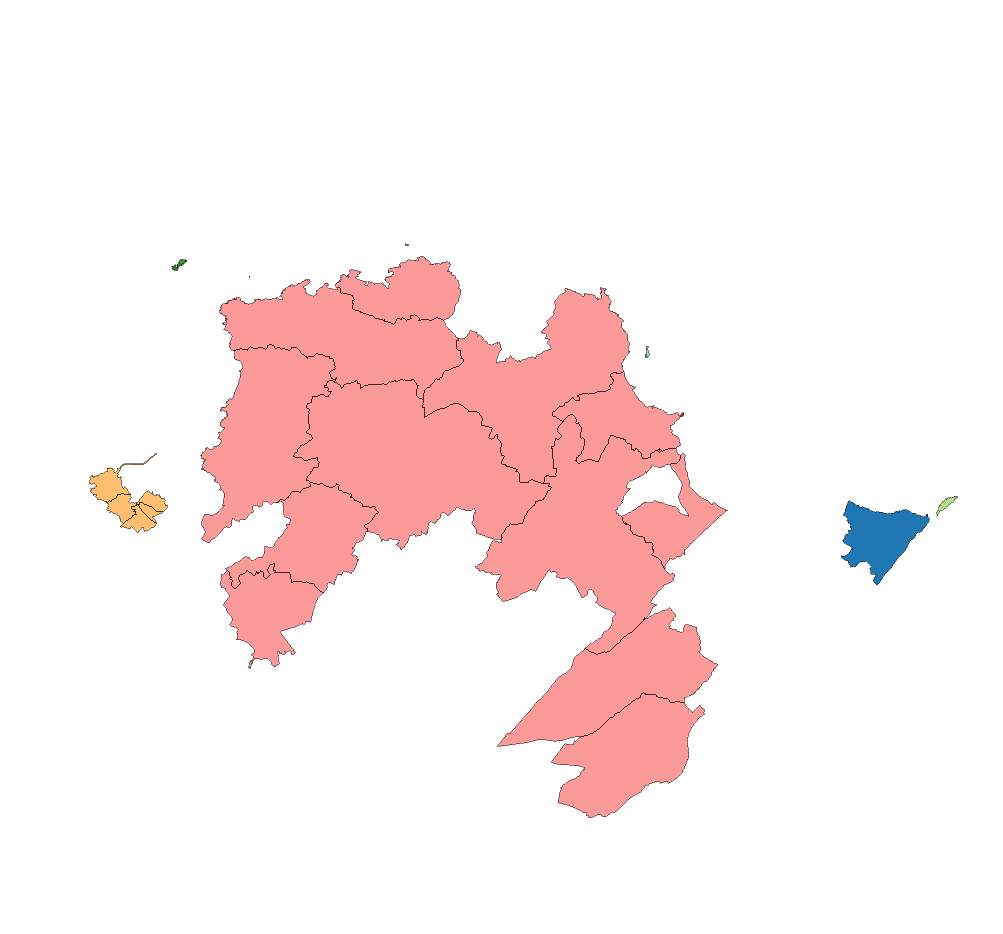
\includegraphics[width=1\linewidth]{images/ch6/contig/11}&
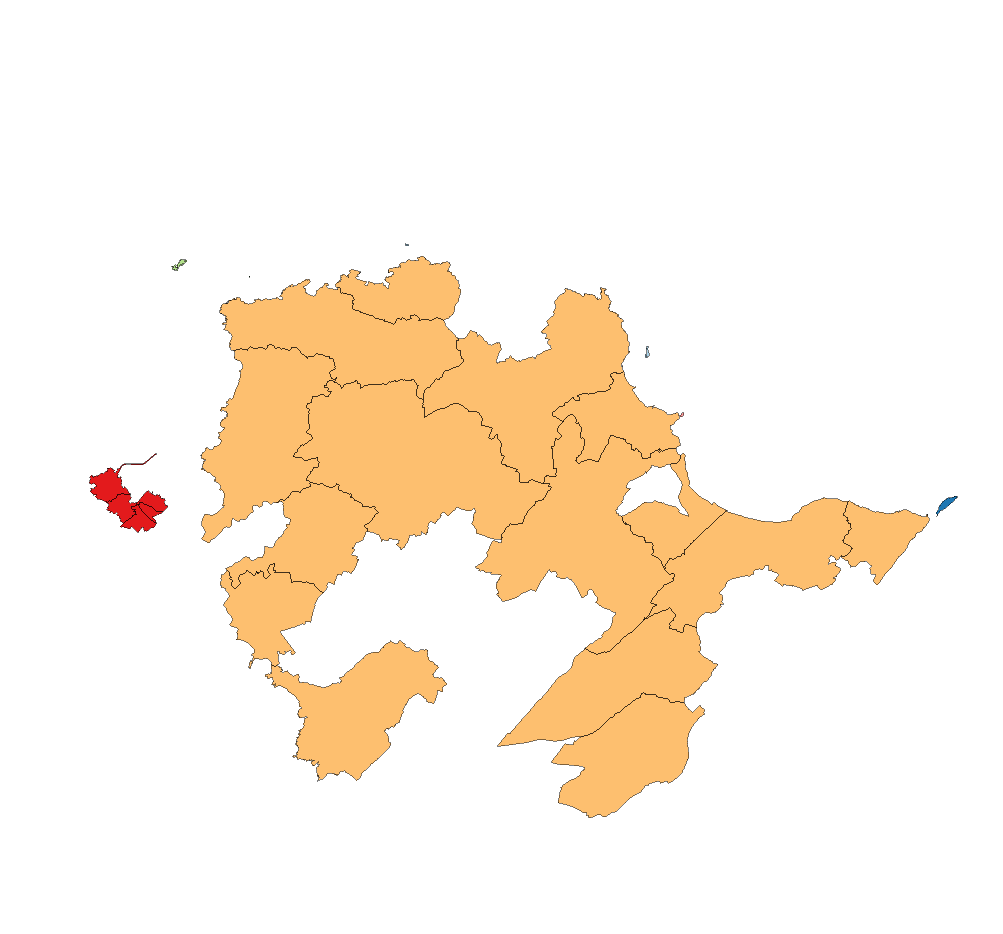
\includegraphics[width=1\linewidth]{images/ch6/contig/12} \\
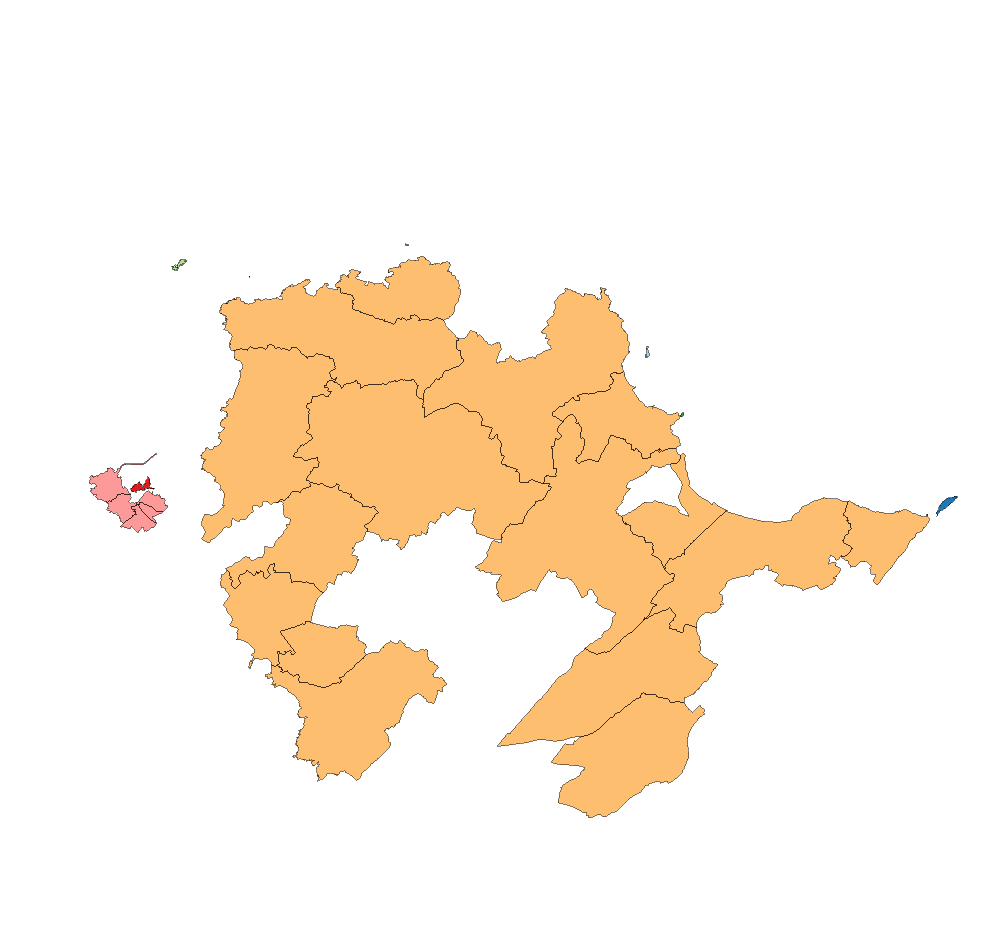
\includegraphics[width=1\linewidth]{images/ch6/contig/13}&
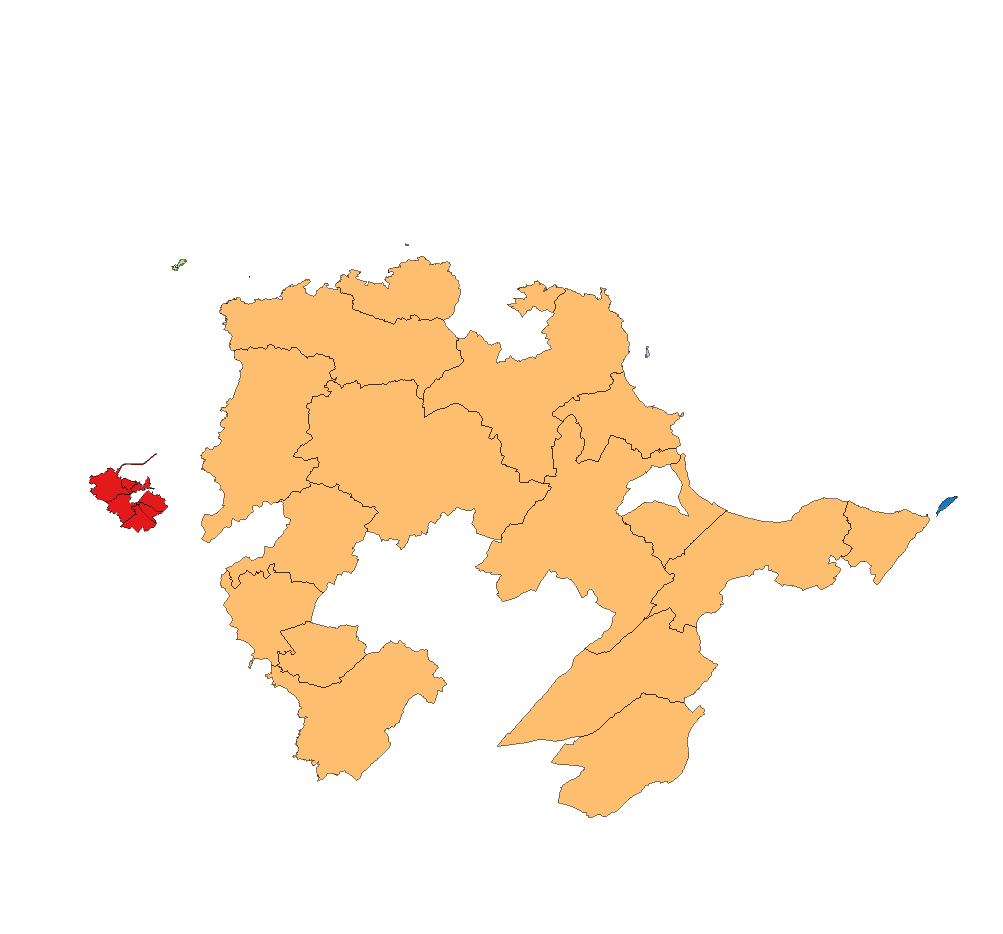
\includegraphics[width=1\linewidth]{images/ch6/contig/14}&
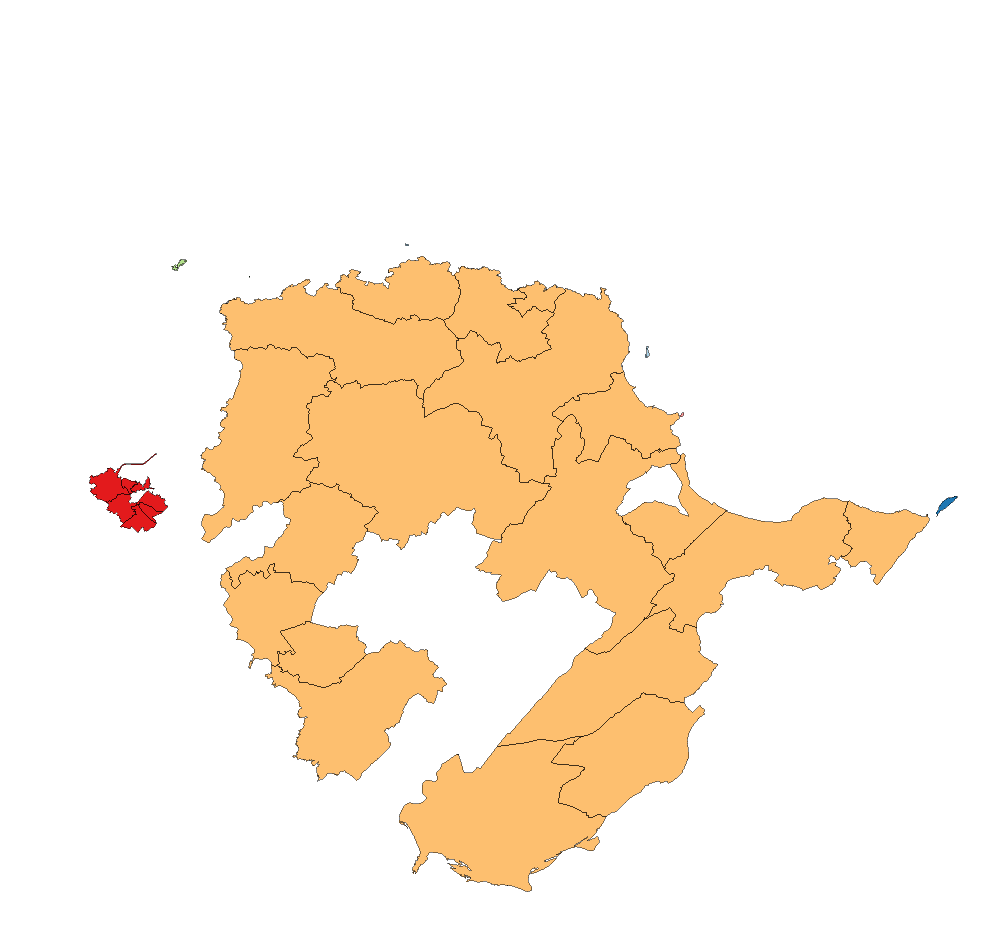
\includegraphics[width=1\linewidth]{images/ch6/contig/15}&
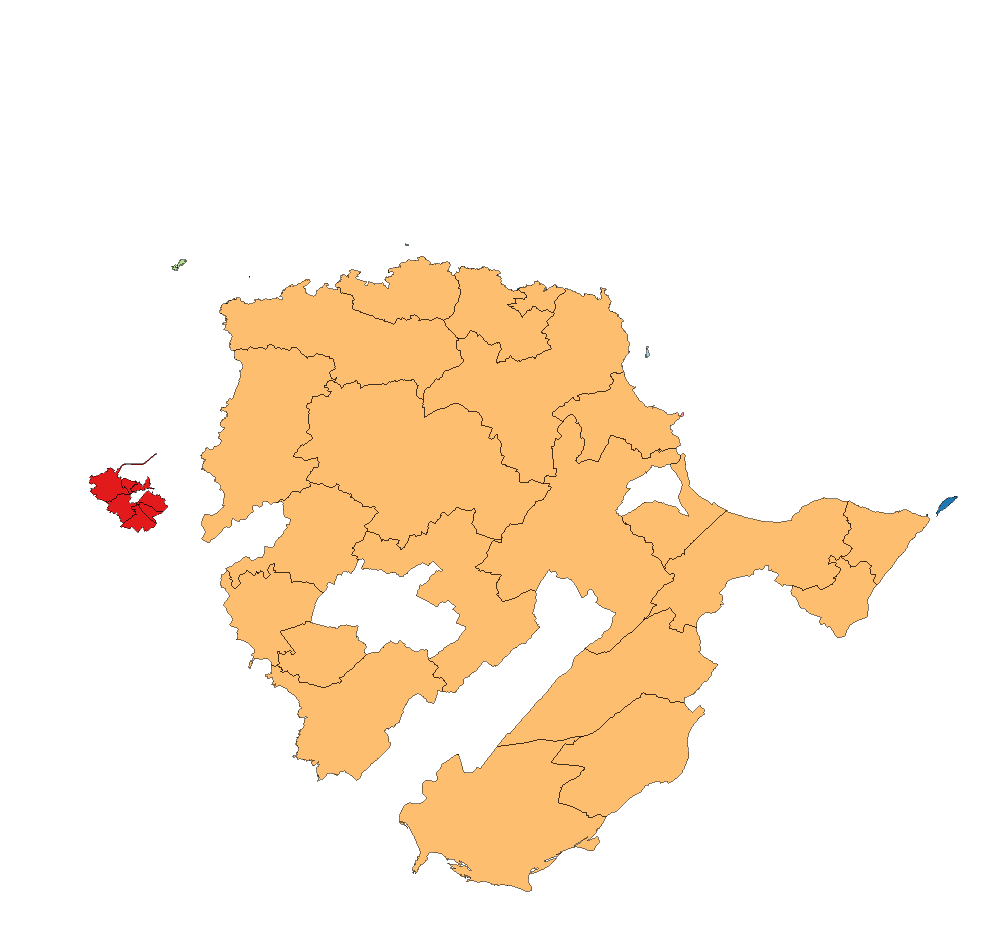
\includegraphics[width=1\linewidth]{images/ch6/contig/16} \\
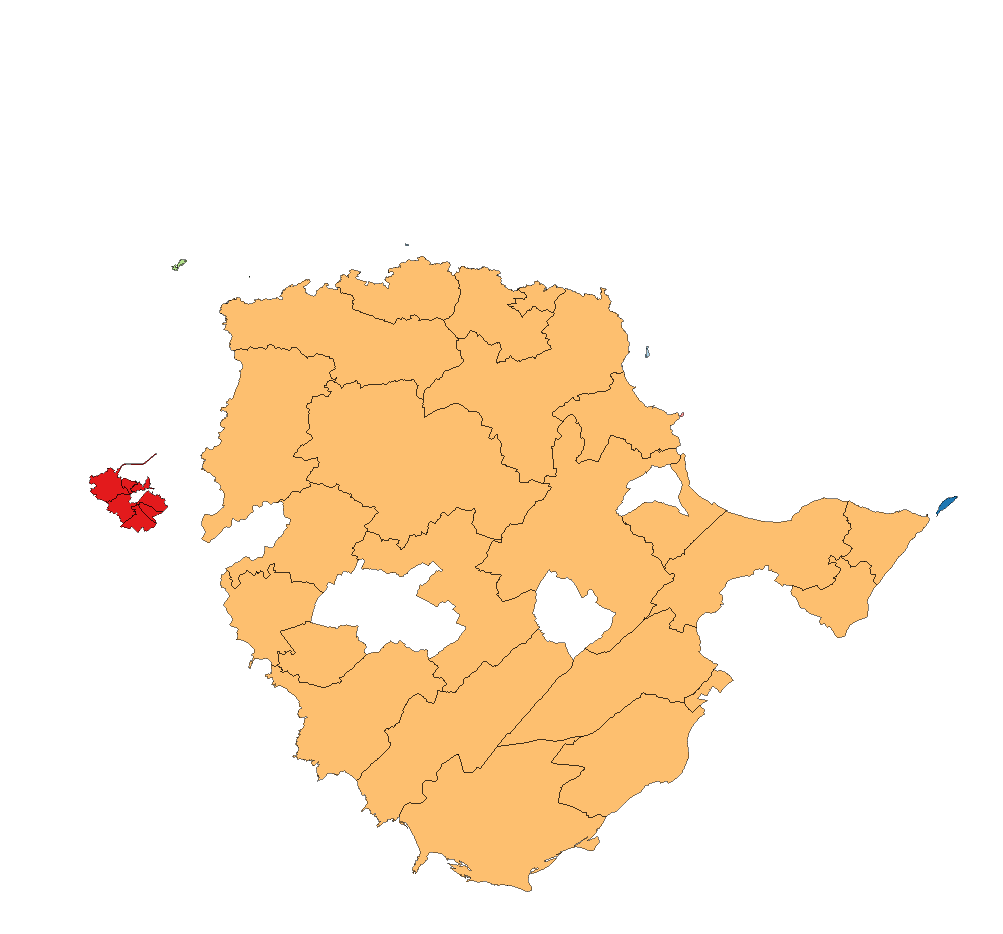
\includegraphics[width=1\linewidth]{images/ch6/contig/17}&
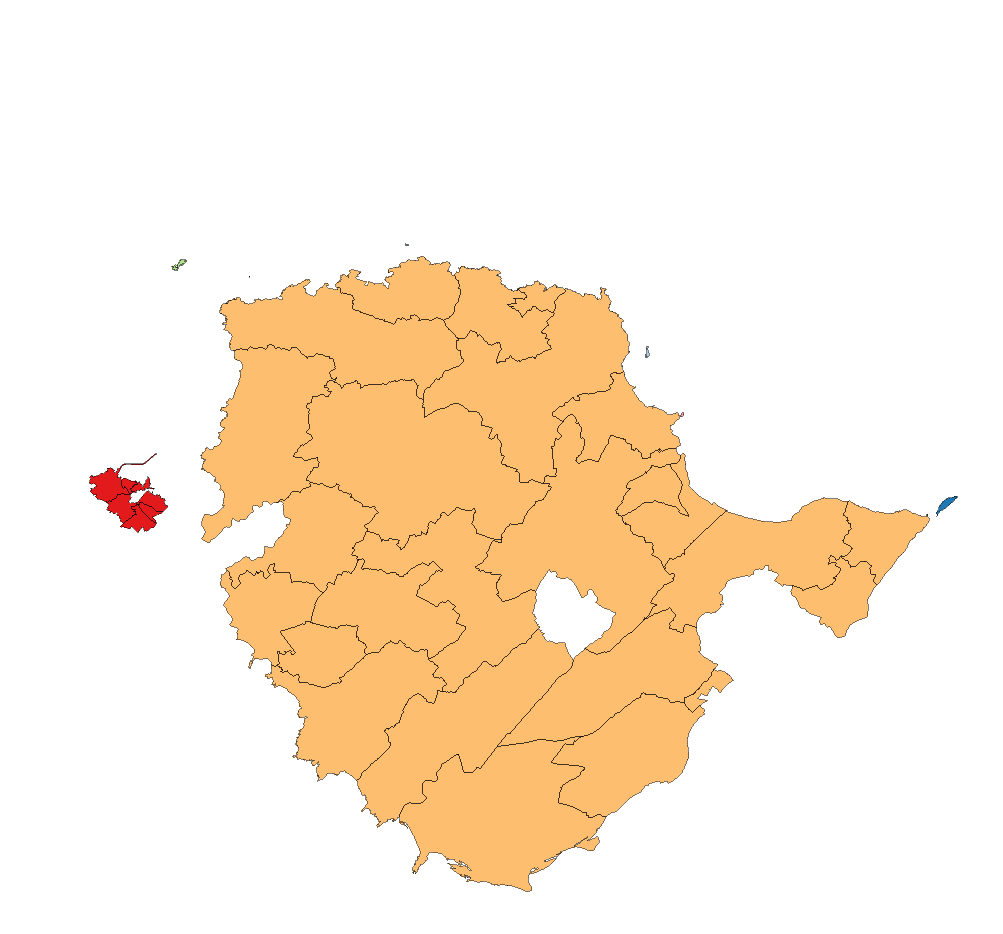
\includegraphics[width=1\linewidth]{images/ch6/contig/18}&
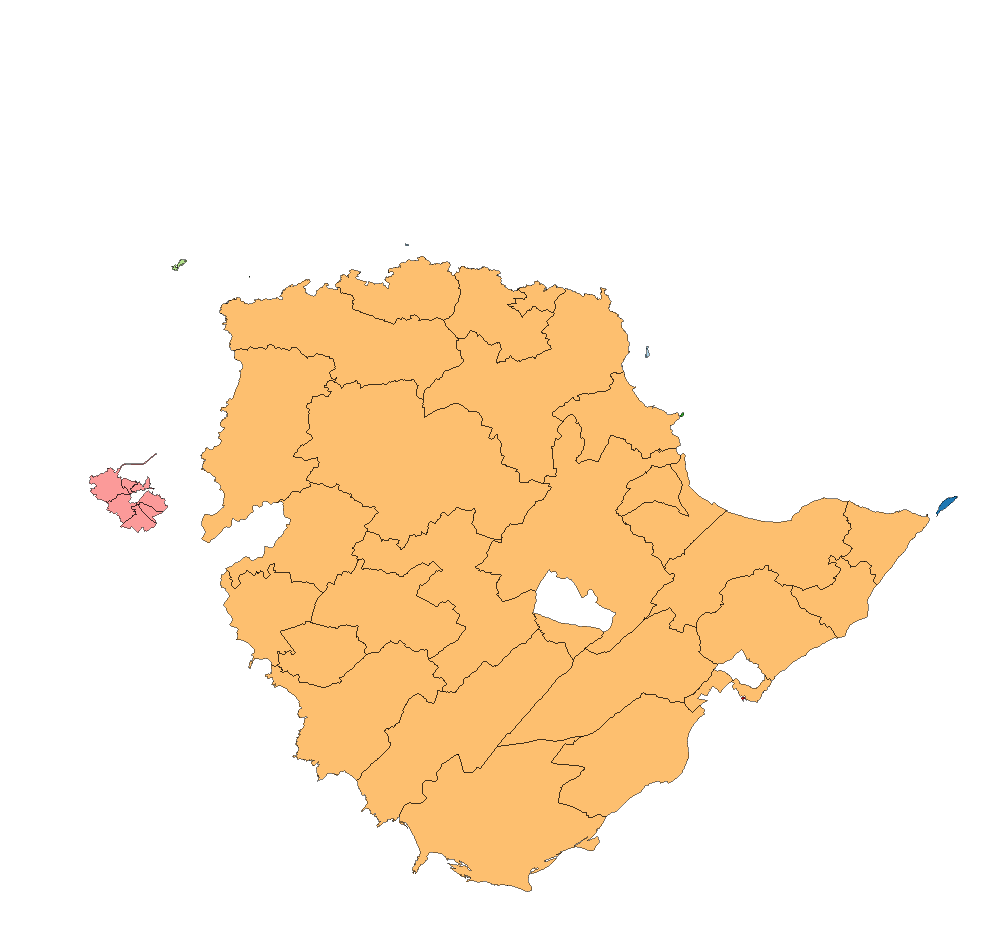
\includegraphics[width=1\linewidth]{images/ch6/contig/19}&
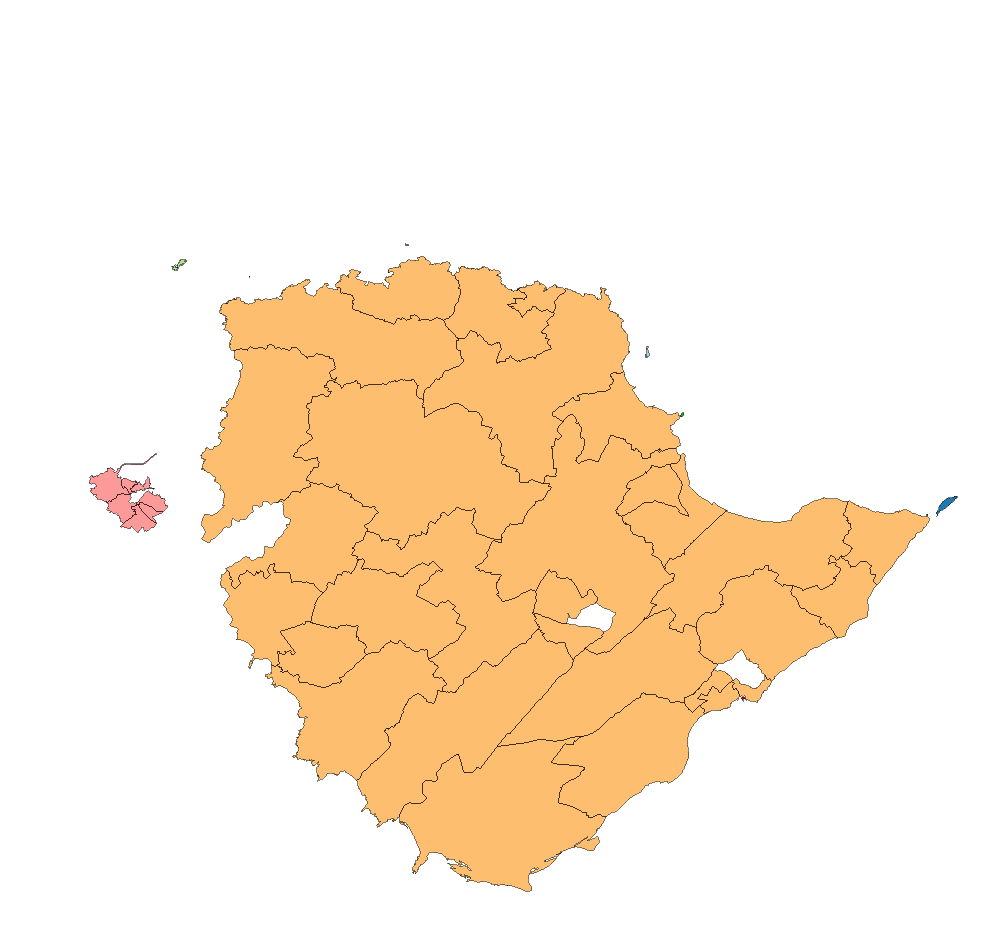
\includegraphics[width=1\linewidth]{images/ch6/contig/20} \\
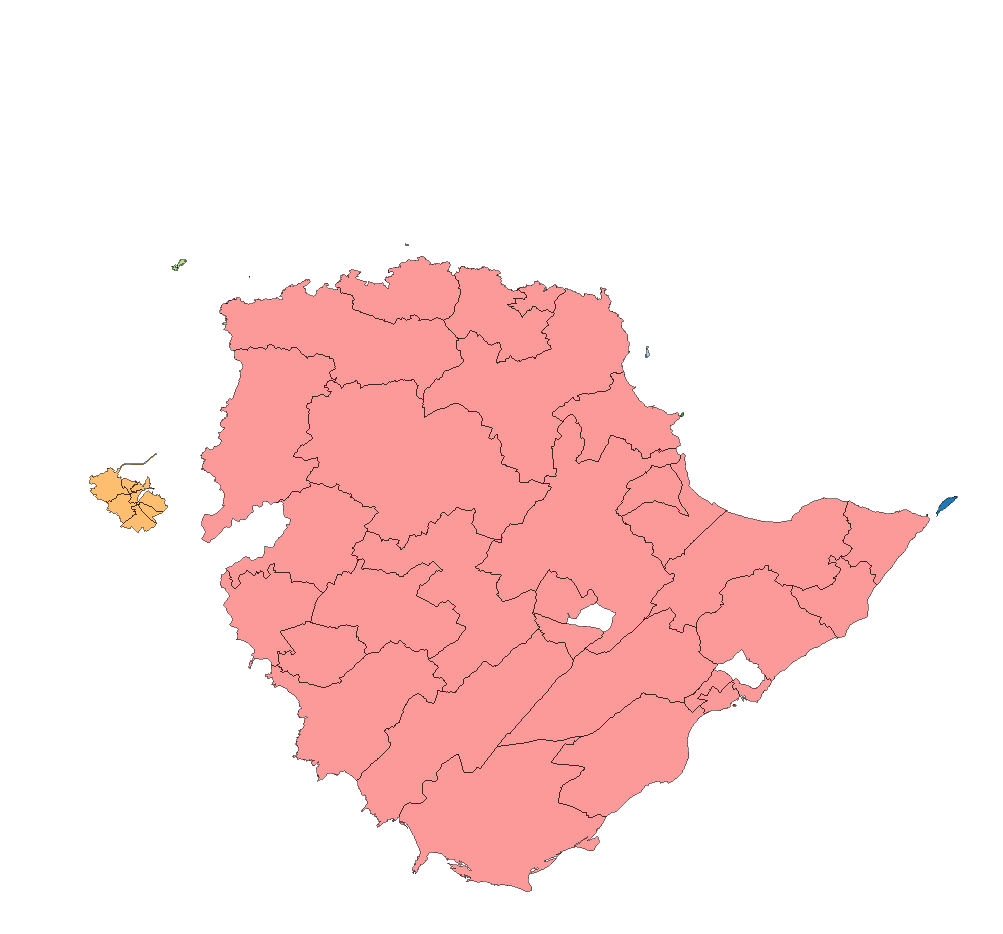
\includegraphics[width=1\linewidth]{images/ch6/contig/21}&
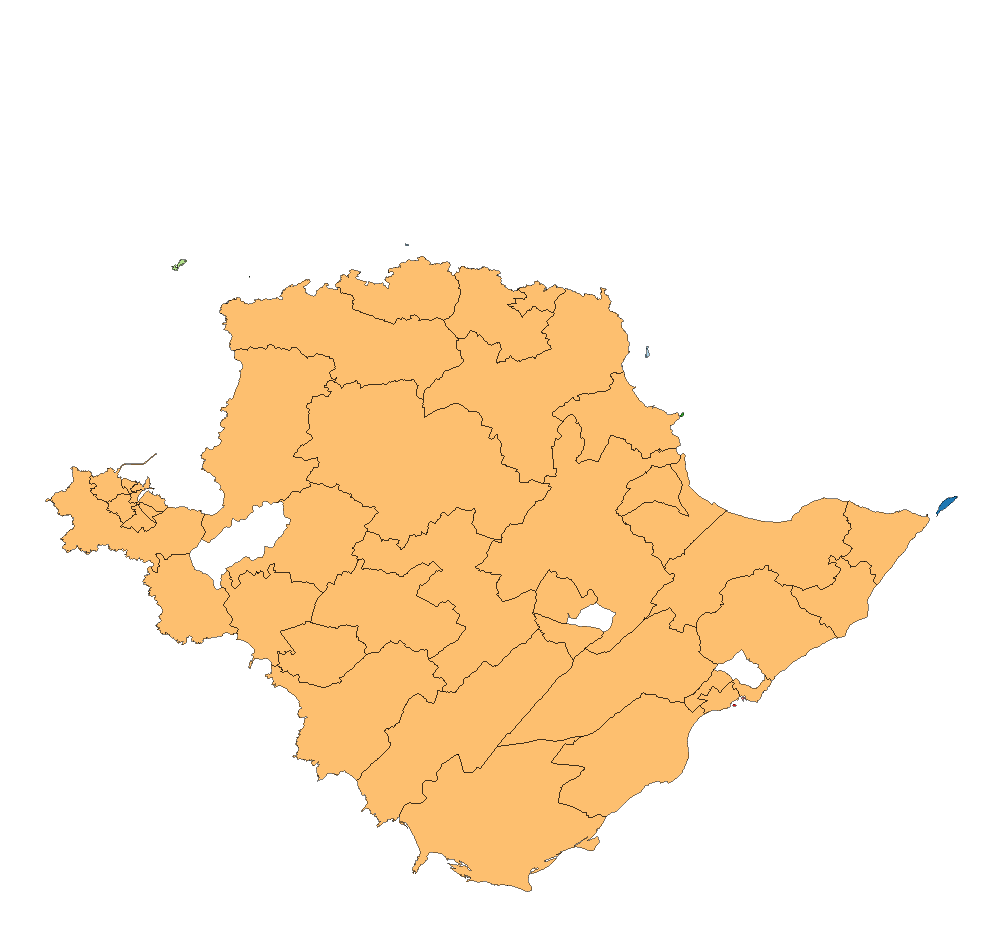
\includegraphics[width=1\linewidth]{images/ch6/contig/22}&
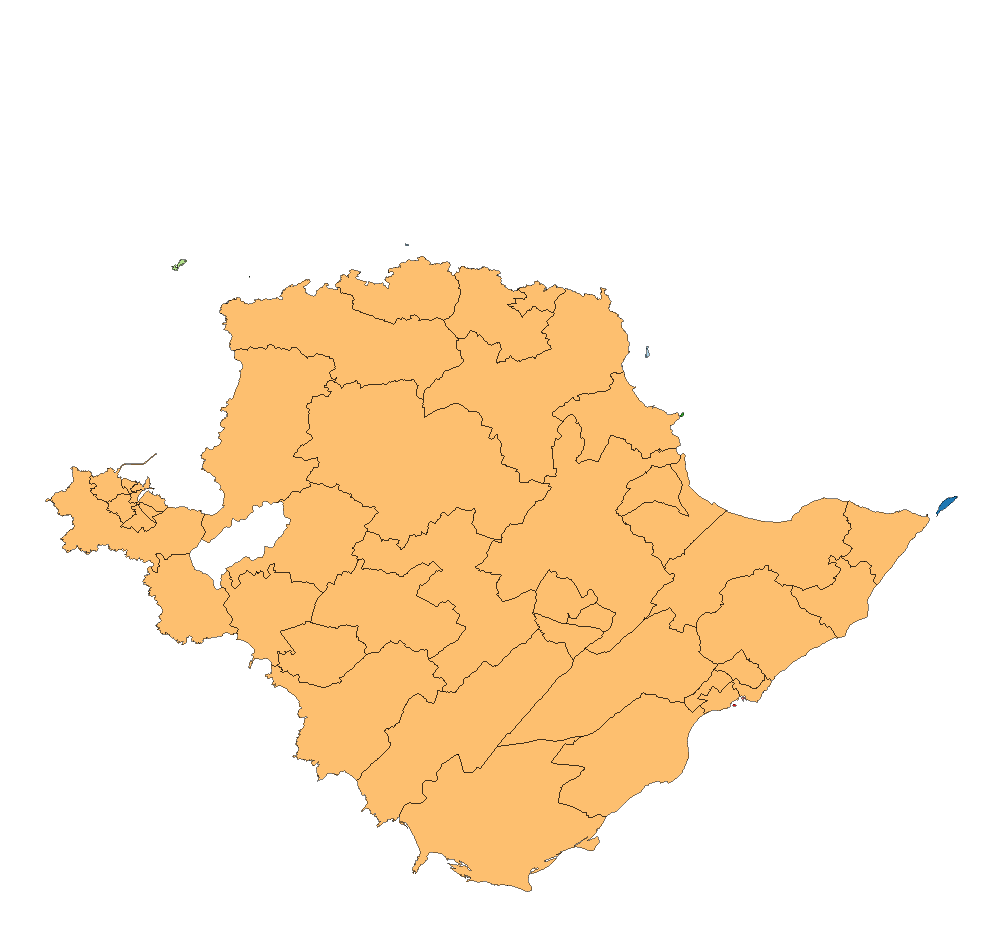
\includegraphics[width=1\linewidth]{images/ch6/contig/23}&
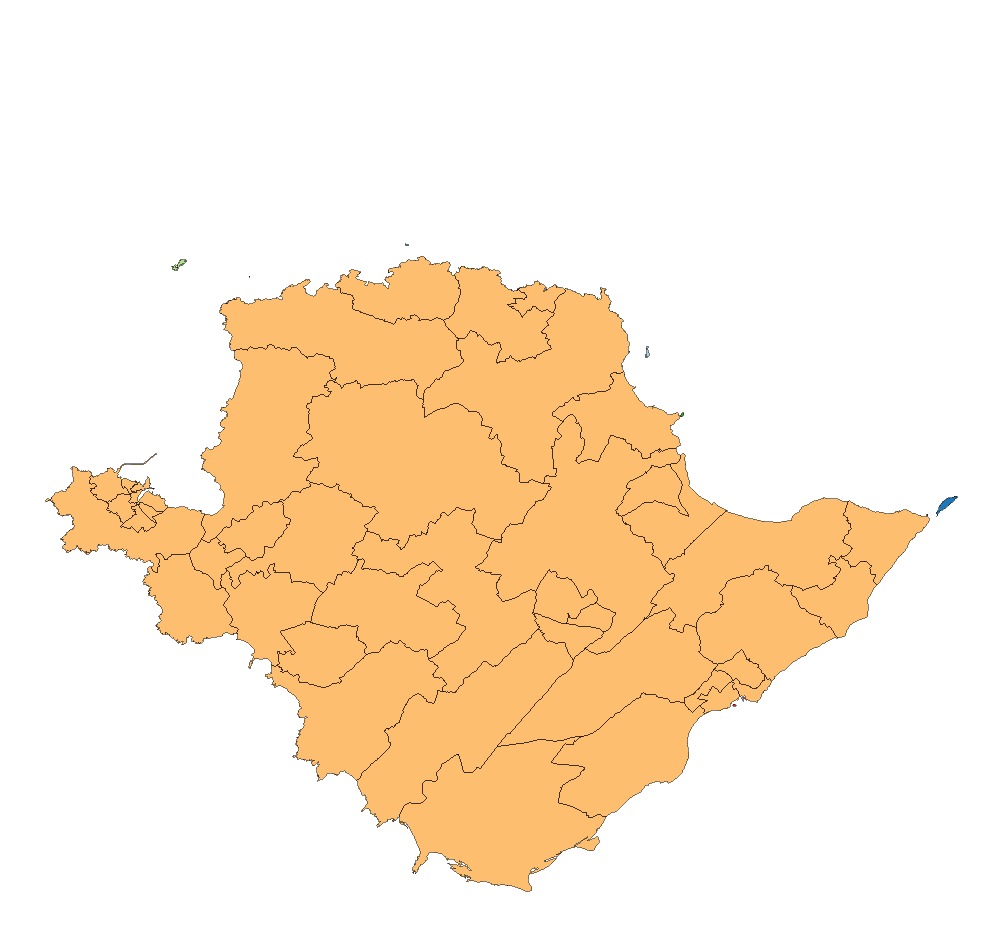
\includegraphics[width=1\linewidth]{images/ch6/contig/24} \\ %24
\end{tabularx}
\caption{A matrix depicting animation slices of the intermediate debug visualization for contiguity debugging. Each color rerpresents a contiguous region. The color considers the number of contiguous regions, and sets the last updated contiguous region to the most recent color. Test data set is relative to Figure \ref{fig:loadingMatrix} for comparison.} \label{fig:contigMatrix}
\end{figure}

\begin{figure}
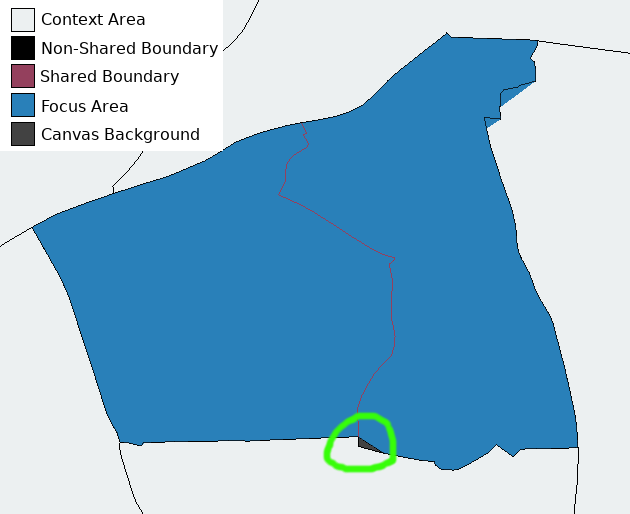
\includegraphics[width=1\textwidth]{images/ch6/WeirdBoundary3}
\caption{ The first instance of shared boundary matching. The red shared boundary refers to the assumed shared boundary. the blue color refers to the focus area, the background cold is represented by the dark grey. The red boundary seems to stop just short of the shared boundary, however there are no vertex points to join at the end causing some error. After seeing this, the algorithm was upgraded to check both sides of a shared boundary and match them using a point-to-line intersection. We highlight the problem with a green circle. }\label{fig:weirdBoundary}
\end{figure} 

\begin{figure}
\includegraphics[width=1\textwidth]{images/ch6/currentProblem}
\caption{The red color represents the assumed shared boundary. The first instance of the T-junction challenge discussed in more detail in Chapter \ref{chap:dcm}.  Using the debug visualization for hierarchy building, along with comparative software tools, we were able to identify the exact vertex point (circled green) that caused the problem. Leading us to re-evaluated the handling of t-junctions. }\label{fig:t-junction}
\end{figure} 

\begin{figure}
\includegraphics[width=1\textwidth]{images/ch6/multipleVoids3}
\caption{This presents a focused step presenting an error that occurred in the processing of the geospatial data. The red line presents the assumed shared boundary, the white presents a context polygon, the grey represents the default background, and the blue signifies the unified polygon. This error was caused by multiple void areas along the shared boundary which result in a unification error. This is because an early version of our algorithm assumed that voids would only occur in singular instances. The fissure made the algorithm believe we rejoined a shared boundary shape, cause most of the boundary to be lost in the unification process, depicted by the straight red line moving off the right size of the canvas which then meets up to complete a loop. Refer to Figure \ref{fig:splitBoundary} for the cause where we match the areas using a green circles.} \label{fig:errorVoids}
\end{figure}

\begin{figure}
\includegraphics[width=1\textwidth]{images/ch6/BoundarySplit2}
\caption{This is a screenshot taken from QGIS to verify an error found in Figure \ref{fig:errorVoids} The polygons contain a strange break in between them which was only visible at a 1:14 scale of the original data set. Something that would be impossible to identify if reviewing the data as an overview image. The white is the background of the software, signifying a lack of any polygonal data. The green circle relates to a point relative to the green circle in Figure \ref{fig:errorVoids}. The void is so thin that we can not clearly identify the all the voids in one image.} \label{fig:splitBoundary}
\end{figure}

\begin{figure}[p]
\begin{tabularx}{1\textwidth}{XXXX}
\includegraphics[width=1\linewidth]{images/ch6/mergeoverall/01}&
\includegraphics[width=1\linewidth]{images/ch6/mergeoverall/02}&
\includegraphics[width=1\linewidth]{images/ch6/mergeoverall/03}&
\includegraphics[width=1\linewidth]{images/ch6/mergeoverall/04} \\
\includegraphics[width=1\linewidth]{images/ch6/mergeoverall/05}&
\includegraphics[width=1\linewidth]{images/ch6/mergeoverall/06}&
\includegraphics[width=1\linewidth]{images/ch6/mergeoverall/07}&
\includegraphics[width=1\linewidth]{images/ch6/mergeoverall/08} \\
\includegraphics[width=1\linewidth]{images/ch6/mergeoverall/09}&
\includegraphics[width=1\linewidth]{images/ch6/mergeoverall/10}&
\includegraphics[width=1\linewidth]{images/ch6/mergeoverall/11}&
\includegraphics[width=1\linewidth]{images/ch6/mergeoverall/12} \\
\includegraphics[width=1\linewidth]{images/ch6/mergeoverall/13}&
\includegraphics[width=1\linewidth]{images/ch6/mergeoverall/14}&
\includegraphics[width=1\linewidth]{images/ch6/mergeoverall/15}&
\includegraphics[width=1\linewidth]{images/ch6/mergeoverall/16} \\
\includegraphics[width=1\linewidth]{images/ch6/mergeoverall/17}&
\includegraphics[width=1\linewidth]{images/ch6/mergeoverall/18}&
\includegraphics[width=1\linewidth]{images/ch6/mergeoverall/19}&
\includegraphics[width=1\linewidth]{images/ch6/mergeoverall/20} \\
\includegraphics[width=1\linewidth]{images/ch6/mergeoverall/21}&
\includegraphics[width=1\linewidth]{images/ch6/mergeoverall/22}&
\includegraphics[width=1\linewidth]{images/ch6/mergeoverall/23}&
\includegraphics[width=1\linewidth]{images/ch6/mergeoverall/24} \\ %24
\end{tabularx}
\caption{A matrix depicting animation slices of the intermediatel debug visualization for hierarchy debugging. The blue color rerpresents the last unified area. Grey polygons represents potential merge candidates, the red line represents the shared boundary found to unify the new area. This matrix presents the overall view of the hierarchy visualization. Relative to Figure \ref{fig:hierarchyFocus} which shows a focus view, for clearer boundary interpretation} \label{fig:hierarchyOverall}
\end{figure}

\begin{figure}[p]
\begin{tabularx}{1\textwidth}{XXXX}
\includegraphics[width=1\linewidth]{images/ch6/mergefocus/01}&
\includegraphics[width=1\linewidth]{images/ch6/mergefocus/02}&
\includegraphics[width=1\linewidth]{images/ch6/mergefocus/03}&
\includegraphics[width=1\linewidth]{images/ch6/mergefocus/04} \\
\includegraphics[width=1\linewidth]{images/ch6/mergefocus/05}&
\includegraphics[width=1\linewidth]{images/ch6/mergefocus/06}&
\includegraphics[width=1\linewidth]{images/ch6/mergefocus/07}&
\includegraphics[width=1\linewidth]{images/ch6/mergefocus/08} \\
\includegraphics[width=1\linewidth]{images/ch6/mergefocus/09}&
\includegraphics[width=1\linewidth]{images/ch6/mergefocus/10}&
\includegraphics[width=1\linewidth]{images/ch6/mergefocus/11}&
\includegraphics[width=1\linewidth]{images/ch6/mergefocus/12} \\
\includegraphics[width=1\linewidth]{images/ch6/mergefocus/13}&
\includegraphics[width=1\linewidth]{images/ch6/mergefocus/14}&
\includegraphics[width=1\linewidth]{images/ch6/mergefocus/15}&
\includegraphics[width=1\linewidth]{images/ch6/mergefocus/16} \\
\includegraphics[width=1\linewidth]{images/ch6/mergefocus/17}&
\includegraphics[width=1\linewidth]{images/ch6/mergefocus/24}&
\includegraphics[width=1\linewidth]{images/ch6/mergefocus/18}&
\includegraphics[width=1\linewidth]{images/ch6/mergefocus/19} \\
\includegraphics[width=1\linewidth]{images/ch6/mergefocus/20}&
\includegraphics[width=1\linewidth]{images/ch6/mergefocus/21}&
\includegraphics[width=1\linewidth]{images/ch6/mergefocus/22}&
\includegraphics[width=1\linewidth]{images/ch6/mergefocus/23} \\ %24
\end{tabularx}
\caption{A matrix depicting time slices of the temporal debug visualization for hierarchy debugging. The blue color rerpresents the last unified area. Grey polygons represents potential merge candidates, the red line represents the shared boundary found to unify the new area. This matrix presents the focus view of the hierarchy visualization. Relative to Figure \ref{fig:hierarchyOverall} which depicts the same visualization using the overall focus to clearly depict progress of the process.} \label{fig:hierarchyFocus}
\end{figure}

\subsection{Hierarchy Building Visualization}
In Chapter \ref{chap:dcm} we state that over 50\% of merges had at least one error case, which is why this section is so important. Our hierarchy building visualization is used to support the identification of a shared boundary between two areas. For each step, we present the newly unified area in blue and every other area that is considered a merge candidate as grey context. This allows us to visualize the hierarchy being built, as well as how it is built. This visualization type allowed us to perceive the majority of errors found during the creation of our algorithm. We present many of the archived errors, in Figures \ref{fig:weirdBoundary}--\ref{fig:splitBoundary}. 

The first error (Figure \ref{fig:weirdBoundary} on Page \pageref{fig:weirdBoundary}) found was identified using our focus time-step, which allowed us to see minor errors in boundary design. This was due to the vertices not always matching up resulting in shared boundaries to be two different topological lengths. After noticing the problem, we added a point-to-line test to identify the closest point to the boundary, and duplicate points to ensure a clean shared boundary.

Although the second error (Figure \ref{fig:t-junction} on Page \ref{fig:t-junction}) is similar to the previous example, the cause is slightly different. We found that we would encounter T-junction challenges during a merge. This is caused when a shared boundary's vertices do not line up with a point that may be used on a later shared boundary. Once identified, we added the option to include point-to-line tests within a shared boundary entirely. Although this would reduce performance time, we rectify this with the ability to load instructions during a second run.

The final case (Figures \ref{fig:errorVoids} \& \ref{fig:splitBoundary} on Pages \pageref{fig:errorVoids} \& \pageref{fig:splitBoundary}) we will look at is caused by what we classify as a fissure, which refers to space between boundary vertices. Although we considered voids as single anomalies along a shared boundary, learning that it was common to have a set of continuous voids (caused by rivers or mountains) made it impossible to ignore these anomalies. This lead us to an extensive re-development of the algorithm, that was used to diagnose the difference between these voids, and a non-shared boundary (refer to Section \ref{sec:complex}).

\section{Intersection Testing for Primatives}
For our algorithm, intersection testing is one of the key areas that we examine when reviewing performance. Two tests, in particular, provide a high frequency of calls, being the bounding box and point-to-line intersection test — the second being used as a deep search into accurate boundary representation, while the first being a filter for clear, non-intersecting polygons. Although there are many methods online to help manage these tests, We did not find a developer-friendly library that managed to guide us with primitive testing. Therefore, we created a small open-source library to test the intersection between five different primitives. The primitives we test are:
\begin{itemize}
\item Point - Defined as an (x, y) coordinate, $p(x,y)$
\item Line Segment - Defined as two points (assumed to be connected), ($p_1,p_2)$)
\item Circle -  Defined by a center point, and a radius, ($p_c,r)$)
\item Triangle - Defined by three points ($p_1,p_2,p_3$)
\item Axis-Aligned Bounding Box (AABB) - Defined by four points, assumed to be aligned.
\end{itemize}

Other than the triangle, which was added for completeness, all of these tests were necessary for software projects. Points are used to present vertices, as well as the mouse pointer, Line Segments are used to test precise boundaries for shared boundary testing, circles are used to test likely collision with glyphs, and axis-aligned bounding boxes are used to test possible collisions with boxes.

\subsection{Motivation}
Generic shape intersection testing is a major component within the algorithm presented in this thesis. We present a table depicting meta data for different tested shape files, and the number of intersection tests we gathered for some of our tests. See Table \ref{tbl:tests}. For this table, we look at the a number of examples that were presented in Chapters \ref{chap:dcm}, \ref{chap:userStudy} \& \ref{chap:MultivariateMaps}. Polygon Count relates to the AABB-to-AABB tests, whilst the vertex count relate to the Point-to-Line tests.

\begin{table}[t]
\footnotesize
\rowcolors{1}{black!10}{white}
\begin{tabularx}{1\linewidth}{|CCC|CCC|}
\hline
\multicolumn{3}{|c|}{\textbf{Meta Data}} & \multicolumn{3}{c|}{\textbf{Intersection Tests}}\\ \hline
ShapeFile Name&Polygon Count&Vertex Count& Point-to-Line (\%) & ABBB-to-AABB (\%)&Total Tests\\ \hline
CCGs& 541	&2,890,934	&5,208,849 (99\%)		&52,284 (1\%)		&5,261,133 \\ 
Ahupuaa Boundaries of Hawaii & 725 & 284,252 & 547,303 (70\%) & 239,024 (30\%) & 786,327 \\
LSOA of Wales & 1,949 &2,417,391 & 4,648,604 (80\%) & 1,175,523 (20\%) & 5,824,127 \\ 
US Counties& 3,134&51,976	&126,841 (6\%)	&2,007,756 (94\%)	&2,134,597 \\ 
Republic of Ireland Electoral Divisions& 4,407		&419,368	&935,468 (16\%)	&4,742,824 (84\%)	&5,678,292\\ 
Germany & 5,385 & 1,456,469 & 6,287,363 (38\%)& 10,093,710 (62\%) & 16,381,073\\
Italy & 8,946 & 966,206 &1,463,588 (4\%) &31,817,661 (96\%)&33,281,249 \\ 
Brazil & 11,181 & 1,288,007 & 6,124,539 (11\%)& 47,995,943 (89\%) & 54,120,482\\ 

\hline
\end{tabularx}
\caption{A table depicting some results for intersecting testing, we depict the two major tests from the examples in Chapter \ref{chap:MultivariateMaps} as well as a few more represented in Chapters \ref{chap:dcm} and \ref{chap:userStudy}.} \label{tbl:tests}
\end{table}

\subsection{Graphical User Interface}
In order to present our header, the files includes a graphical user interface for testing purposes using Qt \cite{Qt}. The user can select any of the primitives to move using their mouse with a dropdown box and create a static primitive to test against using a second  dropdown box. See Figure \ref{fig:inter}.

\subsection{Using Primatives}
The library provides classes for each primitive with basic functionality. The idea behind this library is that testing for intersections is simple. Objects are created or cast into our own primitive objects, and call the function \emph{isIntersecting(Object a, Object b)}, which returns a boolean answer. Although this library appears within our project, we also provide a graphical user interface using Qt to test the library. This enables us to test each primitive against any other primitive with little inconvenience.
\lstinputlisting[language=c++]{src/simpleTest.cpp}

We also give the user access to more information for their own testing. For example, we use a method to test the closest point on a line, to a second point. Rather this allows the user to return that point and make other tests. For example, in our Graphical User Interface, we depict the closestPoint while testing some primitives.

\lstinputlisting[language=c++]{src/closestPoint.cpp}

\subsection{Open Source}
In order to maximize the potential of this library, we upload a public copy to GitHub. The library can be found with the two main headers, the GUI testing project, test cases and full Doxygen documentation. We plan to update this in the future with any performance optimzations, and additional shapes that may be necessary. We also hope to include 3D functionality in the future as well as other shapes in the future. As well as some extra return procedures for the point(s) of intersection, or points clamped outside of the primatives.

\begin{figure}[t]
\subfloat[No Intersection]{
\includegraphics[width=0.44\linewidth]{images/ch6/noInter}}
\subfloat[Intersection]{
\includegraphics[width=0.44\linewidth]{images/ch6/inter}}
\caption{Sample image representing the intersection tester GUI. (a) refers to an example of no intersection occuring, while (b) presents an example of an intersection. When an intersection occurs, the primitives change to green.} \label{fig:inter}
\end{figure}


\section{The Complexities of Identifying a Boundary} \label{sec:complex}
Correctly identifying boundaries was one of the biggest challenges througout the course of the PhD. There were many consideration that were necessary to create a robust procedure which could be used. In order to explain some of these problems, this section will cover some of our previous attempts and the issues that we came across. 

For our first attempt, we implemented a simple vertex matching algorithm. For a merge pair, we check each vertex against every other vertex. Common vertices would be saved to a seperate vertex list and this was used to remove those vertices from both areas. There were two issues with this approach.

\subsection{Unification of Area Pair}

The first issue was that identification of a boundary seemed simple, but unifying the two along this boundary became more difficult. In order to unify the merge pair along their non-shared boundary, it was necessary to identify where in the vertex list the boundaries originated. In order to reconcile this, we made some changes to the algortihm. First, we saved the identity of the beginning and ending points of a shared boundary. This would allow us to recognize where and when we needed to unify the two areas. The second change we made was to control vertex direction. This allows us to increase identification of unification order as following: $P_aOrigin->P_aStart->P_bEnd->P_bStart->P_aEnd->P_aOrigin$. Refer to Figure \ref{fig:attempt1}.
\begin{figure}[b]
\includegraphics[height=0.1\textheight]{images/ch6/attempt1p}
\caption{Our first attempt to unify areas.} \label{fig:attempt1}
\includegraphics[height=0.15\textheight]{images/ch6/attempt2p}
\caption{The final process to unify areas. We re-order the vertex list to sit at the end of a shared boundary.} \label{fig:attempt2}
\end{figure}

The issue with this assumption is with the origin. At this point, we assume that the origin is independant of the shared boundary. This is not the case. A shared boundary can span an arbitrary amount of vertices, and can also be positioned at any within the vertex list. This means that an vertex origin can sit within the shared boundary. In order to rectify this situation, we re-arrange the vertex list of the merge pair in order to pre-emptively sort the vertex list. When we diagnose the end of a shared boundary, we make this the beginning of the non-shared boundary. Refer to Figure \ref{fig:attempt2}.


\subsection{Identifying the Start and End of a Shared Boundary}
Now that we understand why interpreting the start and end of a shared boundary are critical, we can discuss the issues for finding the start and end points of a shared boundary. Attempting to use our previous procedure to identify common vertexes was not appropriate, although we did not fully understand why up to this point. This was due to voids and fissure being left in the non-shared boundary. Because of the frequency of these error, they gained an accumalative effect on further identification processes which caused the algorithm to crash. At this point. we had not implemented debug visualization to aid the cause of the errors. However, we did identify what we considered as rendering errors, points along the shared boundary that were still rendered.

In order to rectify these errors, we moved our selection algorithm to a bi-directional search. The origin, we search both clockwise and non-clockwise. In this case, we can assume that the route can fall under two cases. First the origin sits on a non-shared boundary. If this is the case (Case A), we search bi-directionally if the clockwise search encounters a common vertex, we can present that as the start of the shared boundary whilst the first common vertex in the anticlockwise search will be considered the end of the shared boundary. The second case (Case B) is if we start on a shared boundary. If this is the case, our case can be flipped, where the last common vertex before a non-common vertex in the anti-clockwise direction is the start of the shared boundary, and the last common vertex before a non-common vertex in the clockwise position is the end of the shared boundary. However, this approach falls appart when we add new conditions. Refer to Figure \ref{fig:searchA} for a visual representation.

\begin{figure}[b]
\includegraphics[width=0.6\textwidth]{images/ch6/search}
\caption{The second version of our boundary identifier using a bi-directional search. We identify two cases, Case A refers to the origin (marked by an X) sitting on a non-shared boundary whilst Case B refers to the origin sitting on a shared boundary. The arrows refer to the distance of the direction and length of the clockwise or anti-clockwise search.} \label{fig:searchA}
\end{figure}

The first condition we found was a T-junction. In order to verify a non-common vertex is not part of a shared boundary, we now have to check if this point falls on the line. This increases the complexity of common vertex testing, but the algorithm handles this exception well. The second condition becomes more of an issue. We now find voids which we describe as a spare point on a shared boundary that does not lie on shared boundary line. This complicates Case B, as now we cannot consider the first non-common vertex to accurately depict the start or end of a boundary. For this, we added void checks, to see if the shared boundary contiuned. The other problem with a void is that it now has potential to falsely identify the case. If the origin falls on a void, the algorithm would assume that we now sit within Case A which will present a false boundary selection. This only becomes worse when you consider fissures which act as an arbitrary amount of linked voids, allowing for more oppurtunities for this error to present itself, and nullifies any void checking which could be used to depict error. Finally we find clear examples of voids and fissures having multiple encounters within one shared boundary to complicate this even further. Refer to Figure \ref{fig:searchB} for a visual representation.

\begin{figure}[b]
\includegraphics[width=0.6\textwidth]{images/ch6/search2}
\caption{Errors that occur when voids are considered. We run the same cases and implement voids (highlighted as blue nodes) which causes two distinct errors. As voids can be replaced with fissures, and can be found multiple times. This represents only the simplest cases for error.} \label{fig:searchB}
\end{figure}

In Chapter \ref{chap:dcm}, we discuss the fact that over 50\% of one of our test cases had voids, t-junctions, or fissures, when identifying a shared boundary. This made this a major concern for identifying shared boundaries. We could have cleaned the shapefiles of voids and fissures, however the shape files we work with are considered industry standard. It would be disingenuous to believe that our algorithm was useful when we held the only shapefiles that the algorithm worked with.

In order to rectify this problem, we had to make two assumptions, and attempt a seperate method.
First, we assumed that boundaries between two areas were not split, and were one contiguous boundary. Split shared boundaries between areas are already quite rare, however, we made this assumption due to our focus on scale. Our algorithm's measuring distance is biased towards merging the smallest area with it's smallest neighbour. Even amongst cases where a split boundary could occur, it would be highly irregular for a boundary that caused a split boundary, would not be considered the first area to be merged. 
Our second assumption is that a shared boundary would have a smaller length than a non-shared boundary. It is more likely for this to occur, however just like with our first assumption, we mitigate the chances of our assumption being false by considering the smallest neighbour above others.
